% !TEX root = saveliev_physics_general_course_1.tex
%!TEX TS-program = pdflatex
%!TEX encoding = UTF-8 Unicode
% các textbf được thế thành emph cho phù hợp với bản dịch tiếng việt.-Đã sửa lại thành \textbf vì một số vấn đề.


\chapter{Vật Lý Thống Kê}\label{chap:11}

\section{Một số kiến thứ về lý thuyết về xác suất}\label{sec:11_1}

Giả thử ta có một hệ vĩ mô nào đó\footnote[1]{$\medskip$ Hệ được tạo thành bởi một số khổng các vi hạt (các phân tử, nguyên tử, ion, electron) được gọi là hệ vĩ mô.}. Ta hãy giả thiết rằng một đại lượng $x$nào đó đặc trưng cho hệ có các giá trị rời rạc: 
\begin{equation*}
	x_1, x_2, \ldots, x_i, \ldots, x_k, \ldots, x_s.
\end{equation*}

Ta hãy thực hiện trên hệ một số $N$ rất lớn lần đo đại lượng $x$, bằng cách đưa hệ về cùng một trạng thái ban đầu trước mỗi lần đo. Đáng lẽ để tiến hành các lần đo lặp lại trên cùng một hệ, có thể lấy $N$ hệ như nhai ở cùng một trạng thái và thực hiện đo một lần đại lượng $x$ ở tất cả các hệ đó. Một bộ các hệ như nhau như vậy ở cùng một trạng thái được gọi là \textbf{một tập hợp thống kê}.

Ta giả thử rằng $N_{1}$ phép đo cho kết quả $x_1$, $N_2$ phép đo cho kết quả $x_2$ \ldots, $N_i$ phép đo cho kết quả $x_1$, v.v\ldots ($\sum_{N_i}=N$ là hệ số hệ trong tập hợp). Đại lượng $N_i/N$ được gọi là \textbf{tần số tỷ đối} xuất hiện kết quả $x_i$, còn giới hạn của đại lượng này thu được khi $N$ tiến tới vô cùng, nghĩa là:
\begin{equation}\label{eq:11_1}
	P_i = \lim_{N\to\infty} \frac{N_i}{N}
\end{equation}

\noindent
được gọi là \textbf{xác suất xuất hiện kết quả} $x_i$. Dưới đây, để đơn giản hóa các công thức ta sẽ viết biểu thức cho xác suất dưới dạng $N_i/N$ bằng cách hiểu ngầm rằng ta thực hiện việc chuyển qua giới hạn khi $N\to\infty$.

Vì $\sum_i N_i=N$, nên
\begin{equation}\label{eq:11_2}
	\sum_i P_i = \sum_i \frac{N_i}{N} = 1
\end{equation}

\noindent
nghĩa là tổng các xác suất của tất cả các kết quả khả dĩ của phép đo bằng đơn vị.

Xác suất để thu được kết quả $x_i$ hoặc $x_k$ là bằng
\begin{equation*}
	P_{i\text{ hoặc }k} = \frac{N_i + N_k}{N} = \frac{N_i}{N} + \frac{N_k}{N} = P_i + P_k.
\end{equation*}


\noindent
Vậy ta đi tới \textbf{định lý cộng các xác suất};định lý đó khẳng định rằng
\begin{equation}\label{eq:11_3}
	P_{i\text{ hoặc }k} = P_i + P_k.
\end{equation}

Giả thử hệ được đặc trưng bàng cac giá trị của hai đại lượng $x$ và $y$, thêm vào đó cả hai đại lượng đều có thể nhận giá trị rời rạc mà xác suất xuất hiện chúng là bằng
\begin{equation*}
	P(x_i) = \frac{N(x_i)}{N},\quad P(y_k) = \frac{N(y_k)}{N}.
\end{equation*}

\noindent 
Ta hãy tìm xác suất $P(x_i,y_k)$ để với một phép đo nào đó đối với $x$ sẽ thu được kết quả $x_i$, còn đối với $y$ là kết quả $y_k$. Người ta thu được kết quả $x_i$ trong số lần đo bằng $N(x_i)=P(x_i)N$. Nếu giá trị của đại lượng $y$ không phù thuộc vào giá trị của đại lượng $x$ thì người ta sẽ thu được kết quả $y_k$ đồng thời với $x_i$ trong một số trường hợp bằng
\begin{equation*}
	N(x_i,y_k) = N(x_i) P(y_k) = [P(x_i) N] P(y_k)
\end{equation*}

\noindent
(đối với $y$ thì $N(x_i)$ đóng vai trò của $N$). Xác suất cần tìm bằng
\begin{equation*}
	P(x_i,y_k) = \frac{N(x_i,y_k)}{N} = P(x_i) P(y_k).
\end{equation*}

\noindent
Ta đã đi tới \textbf{định lý về nhân các xác suất}, theo định lý này  \textit{xác suất xuất hiện đồng thời các sự kiện độc lập thống kê là bằng tích các xác suất của các sự kiện đó}:
\begin{equation}\label{eq:11_4}
	P(x_i,y_k) = P(x_i) P(y_k).
\end{equation}

Khi biết xác suất xuất hiện các kết quả khác nhau của phép đo, có thể tìm được các giá trị trung bình của tất cả các kết quả. Theo định nghĩa của giá trị trung bình:
\begin{equation}\label{eq:11_5}
	\average{x} = \frac{1}{N}\sum_i N_i x_i = \sum_i P_i x_i.
\end{equation}

Ta hãy mở các kết quả thu được cho các trường hợp khi đại lượng $x$ đặc trưng cho hệ có thể nhận một loạt giá trị liên tục từ 0 đến $\infty$.Trong trường hợp này người ta nói rằng đại lượng $x$ có phổ các giá trị dày đặc(hoặc liên tục) (trong trường hợp trước phổ các giá trị là gián đoạn).

Ta hãy lấy một đại lượng rất nhỏ $a$ (chẳng hạn, $a=\num{e-6}$) và tìm số lần đo $\Delta N_0$ với $0<x<a$, $\Delta N_0$ với $a<x<2a$, \ldots, $\Delta N_x$ với kết quả các lần đo ở trong khoảng từ $x$ đến $x+a$, v.v, \ldots. Xác suất để kết quả các lần đo ở trong khoảng từ không đến $a$ là bằng $\Delta P_0=\Delta N_0/N$, trong khoảng từ $a$ đến $2a$ là bằng $\Delta P_1= \Delta N_1/N$, \ldots, trong khoảng từ $a$ đến $(x+a)$ là bằng $\Delta P_x=\Delta N_x/N$. Ta vẽ trục $x$ và đặt ở phía trên nó các dải có bề rộng $a$ và chiều cao $\Delta P_x/a$ (\fig{11_1}a). Giản đồ hình cột thu được gọi là \textbf{biểu cột} hoặc \textbf{biểu đồ tần suất}\footnote[1]{$\medskip$ Biểu đồ tần suất còn được gọi là tổ chức đồ.}. Diện tích của một dải mà mép trái của nó có tọa độ $x$ là bằng $\Delta P_x$, còn diện tích của tất cả các biểu đồ tần suất là bằng đơn vị (xem \eqn{11_2}).
%trong sách việt thì gọi chung là tổ chức đồ nhưng mình dịch là biểu đồ tần suất hoặc biểu đồ cột như trong sách gốc.
% tổ chức đồ giờ đây sẽ dịch là biểu đồ tần suất.

\begin{figure}[!htb]
	\begin{center}
		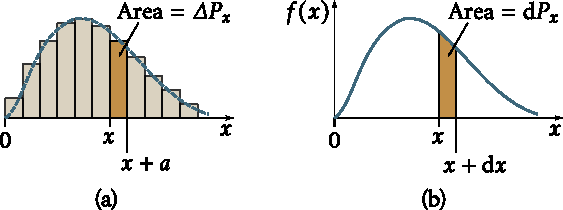
\includegraphics[scale=1.0]{figures/ch_11/fig_11_1.pdf}
		\caption[]{}
		\label{fig:11_1}
	\end{center}
	\vspace{-0.8cm}
\end{figure}


Biểu đồ tần suất đặc trưng một cách cụ thể xác suất thu được các kết quả đo bao hàm trong các khoảng khác nhau có bề rộng $a$. Bề rộng của khoảng $a$ càng nhỏ thì sự phân bố xác suất của các giá trị của đại lượng $x$ sẽ được đặc trưng càng chi tiết hơn.Tại giới hạn khi $a\to 0$, đường bậc thang giới hạn biểu đồ tần suất trở thành một đường cong trơn (\fig{11_1}b). Hàm $f(x)$ xác định đường cong này một cách giải tích được gọi là \textbf{hàm phân bố các xác suất}.  

Theo cách vẽ đường cong phân bố, diện tích của cột có bề rộng $\deriv{x}$ (xen hình \fig{11_1}b) là bằng xác suất để kết quả đo rơi vào các phạm vi từ $x$ đến $x+\deriv{x}$. Nếu ký hiệu xac suất này là $\deriv{P_x}$, có thể viết
\begin{equation}\label{eq:11_6}
	\deriv{P_x} = f(x)\,\deriv{x}.
\end{equation}

\noindent
Chỉ số ``x'' ở $\deriv{P}$ chỉ xác suất đối với khoảng mà mép trái của nó nằm tại điểm có tọa độ $x$ được chú ý đến. Diện tích được giới hạn bởi đường cong phân bố cũng như diện tích của biếu đồ tần số, là bằng đơn vị. Điều này có nghĩa là
\begin{equation}\label{eq:11_7}
	\int f(x)\,\deriv{x} = \int \deriv{P_x} = 1.
\end{equation}

\noindent

Việc lấy tích phân được thực hiện theo toàn khoảng các giá tị khả dĩ của đại lượng $x$. Công thức~\eqref{eq:11_7} là tương tự với công thức \eqn{11_2}.

Biết hàm phân bố $f(x)$ có thể tìm giá trị trung bình của các kết quả đo đại lượng $x$. Trong $\deriv{N_x}=N\,\deriv{P_x}$ trường hợp, ta thu được kết quả bằng $x$. Tổng các kết quả  như vậy được xác định bằng biểu thức $x\deriv{N_x}$. Tổng của tất cả các kết quả khả dĩ là bằng $\int x\,\deriv{N_x}=\int xN\,\deriv{P_x}$. Chia tổng này cho số lần đo $N$, ta thu được giá trị trung bình của đại lượng $x$:
\begin{equation}\label{eq:11_8} 
	\average{x} = \int x\,\deriv{P_x}.
\end{equation}

\noindent
Công thức này tương tự với công thức \eqn{11_5}.

Thay \eqn{11_6} đối với $\deriv{P_x}$ vào \eqn{11_8}, ta đi tới công thức
\begin{equation}\label{eq:11_9}
	\average{x} = \int x f(x)\,\deriv{x}.
\end{equation}

Các lập luận tương tự cho giá trị trung bình của một hàm $\varphi(x)$ nào đó có thể tính theo công thức 
\begin{equation}\label{eq:11_10}
	\average{\varphi(x)} = \int \varphi(x) f(x)\,\deriv{x}.
\end{equation}

\noindent
Chẳng hạn,
\begin{equation}\label{eq:11_11}
	\average{x^2} = \int x^2 f(x)\,\deriv{x}.
\end{equation}

\section{Tính chất của chuyển động nhiệt của các phân tử}\label{sec:11_2}

Nếu chất khí ở trạng thái cân bằng thì các phân tử chuyển động một cách hoàn toàn mất trật tự, hỗn loạn. Tất cả các hướng chuyển động là đồng xác suất, một trong các hướng này không thể có ưu thế hơn các hướng khác. Các vận tốc của các phân tử có thể rất khác nhau về độ lớn. Trong mỗi va chạm với các phân tử khác, độ lớn của vận tốc của phân tử đã cho nói chung phải bị biến đổi, thêm vào đó nó có thể tăng lên cũng như giảm xuống với xác suất bằng nhau.

Sự biến đổi các vận tốc của các phân tử khi va chạm xảy ra một cách ngẫu nhiên. Có thể xảy ra là một phân tử nào đó sau một loạt va chạm kế tiếp nhau sẽ thu năng lượng từ các phân tử đã va chạm với nó, do đó năng lượng của nó trọi hơn giá trị trung bình $\average{\varepsilon}$ rất nhiều. Tuy vây, ngay cả nếu tưởng tượng một trường hợp hoàn toàn kỳ lạ mà trong đó tất cả các phân tử khí dừng lại, truyền năng lượng của phân tử này, và do đó cả vận tốc của nó sẽ là hữu hạn. Vậy vận tốc của các phân tử khí nói chung không thể có các giá trị bắt đầu từ $\ab{v}{max}$ nào đó đến $\infty$. Nếu chú ý rằng các quá trình mà chúng đã có thể dẫn đến sự tập trung vào một phân tử một phần năng lượng tổng cộng đáng kể của tất cả các phân tử là có xác suất nhỏ, thì có thể khẳng định rằng các vận tốc rất lớn so với giá trị trung bình có thể được thực hiện một cách cực kỳ hiếm. Cũng đúng như vậy, trong thực tế người ta loại trừ rằng do các va chạm, vận tốc của phân tử trở nên đúng bằng không. Do đó các vận tốc rất nhỏ và rất lớn so với giá trị trung bình là có xác suất nhỏ, thêm vào đó xác suất của giá trị $v$ đã cho tiến tới không khí $v\to0$ cũng như khi $v\to\infty$. Từ điều đã nói suy ra rằng các vận tốc của các phân tử về căn bản được nhóm lại ở gần một giá trị có xác suất lớn nhất nào đó.

\begin{figure}[!htb]
	\begin{center}
		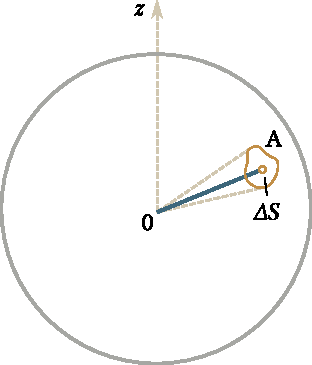
\includegraphics[scale=0.95]{figures/ch_11/fig_11_2.pdf}
		\caption[]{}
		\label{fig:11_2}
	\end{center}
	\vspace{-0.8cm}
\end{figure}

Có thể làm cho sự hỗn loạn của chuyển động các phân tử trở thành rõ ràng bằng phương pháp sau đây. Ta bao quanh điểm $O$ bằng một quả cầu có bán kính $r$ tùy ý (\fig{11_2}). Một điểm A bất kỳ trên quả cầu này xác định hướng từ $O$ đến A. Do đó các hướng mà theo đó các phân tử khí chuyển động tại một thười điểm nào đó có thể được cho bằng các điểm trên hình cầu. Sự đồng khả năng của tất cả các hướng dẫn tới điều là các điểm biểu diễn các hướng chuyển động của các phân tử được phân bố trên hình cầu với mật độ không đổi bằng số phân tử được xét $N$ chia cho bề mặt hình cầu $4\pi r^2$. Các va chạm đều dẫn đến sự biến đổ các hướng chuyển động của các phân tử, vì thế các vị trí của $N$ điểm trên hình cầu bị biến đổi liên tục. Tuy nhiên do sự hỗn loạn của chuyển động, mật độ của các điểm tại một vị trí bất kỳ của hình cầu là luôn luôn không đổi. 

Số các hướng khả dĩ trong không gian là vô cùng lớn. Ngay tại mỗi thời điểm một số hữu hạn các hướng lớn bằng số lượng phân tử được khảo sát được thực hiện. Do đó cách đặt vấn đề về số phân tử có hướng chuyển động đã cho (được mô tả bằng một điểm trên hình cầu) đã bị mất ý nghĩa. Thật vậy, vì số hướng khả dĩ là lớn vô hạn, còn số phân tử là hữu hạn nên xác suất để thậm chí một phân tử bay bắt đầu theo một hướng được xác định là bằng không. Cách nêu vấn đề hợp lý là, có bao nhiêu phân tử chuyển động theo các hướng gần với hướng đã cho (được xác định bằng một điểm A trên hình cầu). tất cả các điểm của yếu tố bề mặt hình cầu $\Delta S$ được lấy tại lân cận điểm A (\fig{11_2}) ứng với các hướng như vậy. vì các điểm biểu diễn các hướng chuyển động của các phân tử được phân bố đều theo mặt cầu nên số lượng các điểm trong phạm vị $\Delta S$ là bằng
\begin{equation}\label{eq:11_12}
	\Delta \ab{N}{A} = N\frac{\Delta S}{4\pi r^2}.
\end{equation}

\noindent
Chỉ số A ở $\Delta N$ chỉ rõ một điều là ta chú ý tới các phân tử hướng chuyển động gần hướng được xác định bởi điểm A.

Tỷ số $\Delta S/r^2$ là góc khối $\Delta \Omega$ quét trên diện tích $\Delta S$. Do đó có thể viết công thức \eqn{11_12} như sau:
\begin{equation}\label{eq:11_13}
	\Delta \ab{N}{A} = N\frac{\Delta\Omega}{4\pi}.
\end{equation}

\noindent
Có thể cho hướng của đoạn thẳng $O$A nhờ góc cực $\theta$và góc phương vị $\varphi$ (\fig{11_3}). Do đó có thể đặc trưng  các hướng chuyển động của các phân tử, bằng cách cho các giá trị của các góc $\theta$ và $\varphi$ đối với mỗi phần tử, bằng cach cho các giá trị từ một hướng cố định $O$z nào đó (có thể lấy, chẳng hạn, hướng của pháp tuyến với bề mặt bình chứa khí làm hướng như thế) và vẽ mặt phẳng $P_0$ qua nó.
\begin{figure}[!htb]
	\begin{minipage}[t]{0.5\linewidth}
		\begin{center}
			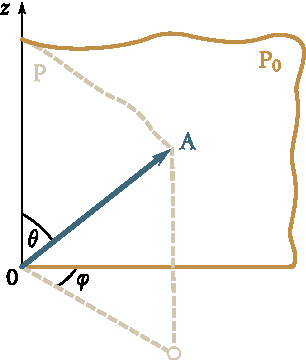
\includegraphics[scale=1.0]{figures/ch_11/fig_11_3.pdf}
			\caption[]{}
			\label{fig:11_3}
		\end{center}
	\end{minipage}
	\hspace{-0.05cm}
	\begin{minipage}[t]{0.5\linewidth}
		\begin{center}
			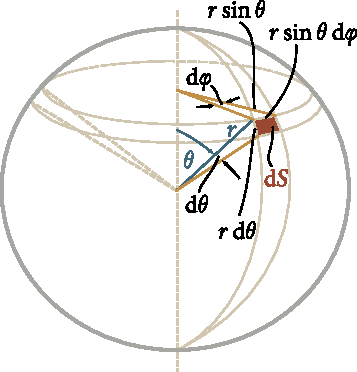
\includegraphics[scale=1.0]{figures/ch_11/fig_11_4.pdf}
			\caption[]{}
			\label{fig:11_4}
		\end{center}
	\end{minipage}
	\vspace{-0.4cm}
\end{figure}
Ta bao quanh gốc tọa độ $O$ bằng một hình cầu bán kính $r$ và tìm được yếu tố $\deriv{S}$ của hình cầu ứng với số gia $deriv{\theta}$ và $\deriv{\theta}$ của các góc $\theta$ và $\varphi$ (\fig{11_4}). Yếu tố được xét là một hình chữ nhật với các cạnh của $r\deriv{\theta}$ và $rsin(\theta)\deriv{\varphi}$. Vậy
\begin{equation}\label{eq:11_14}
	\deriv{S} = r^2 \sin\theta\,\deriv{\theta}\,\deriv{\varphi}.
\end{equation}

\noindent
Biểu thức nhận được cho ta yếu tố bề mặt $r=\text{const}$ trong hệ tọa độ cầu.
Chia biểu thức \eqn{11_4} cho $r^2$, ta tìm được yếu tố góc khối ứng với các khoảng của các góc từ $\theta$ đến $\theta+\deriv{\theta}$ và từ $\varphi$ dến $\varphi+\deriv{\varphi}$:
\begin{equation}\label{eq:11_15}
	\deriv{\Omega_{\theta,\varphi}} = \sin\theta\, \deriv{\theta} \,\deriv{\varphi}.
\end{equation}
Hai hình cầu với các bán kính $r$ và $r+\deriv{r}$, hai hình nón với các góc $\theta$ và $\theta+\deriv{\theta}$ và hai mặt phẳng tạo với $P_0$ các góc $\varphi$ và $\varphi+\deriv{\varphi}$ sẽ tách ra trong không gian một hình hộp chữ nhật với các cạnh $r\deriv{\theta}$, $rsin(\theta)\deriv{\varphi}$ và $\deriv{r}$ (xem \fig{11_4}). Thể tích của hình hộp này
\begin{equation}\label{eq:11_16}
	\deriv{V} = r^2\sin\theta\, \deriv{r}\, \deriv{\theta} \,\deriv{\varphi}
\end{equation}

\noindent
là một yếu tố thể tích trong hệ tọa độ cầu (thể tích ứng với số gia của các tọa độ $r$, $\theta$, $\varphi$ là $\deriv{r}$, $\deriv{\theta}$, $\deriv{\varphi}$.

Trong \eqn{11_13} chuyển từ các delta sang các vi phân và thay thế biểu thức \eqn{11_15} đối với $\deriv{\Omega}$, ta đi tới công thức:
\begin{equation}\label{eq:11_17}
	\deriv{N_{\theta,\varphi}} = N\frac{\deriv{\Omega_{\theta,\varphi}}}{4\pi} = N\frac{\sin\theta\,\deriv{\theta}\,\deriv{\varphi}}{4\pi}.
\end{equation}

\noindent
Các chỉ số $\theta$ và $\varphi$ trong $\deriv{N}$ chỉ rõ rằng ta chú ý đến các phân tử mà các hướng chuyển động của chúng ứng với các khoảng của các góc từ $\theta$ đến $\theta+\deriv{\theta}$ và từ $\varphi$ đến $\varphi+\deriv{\varphi}$.

\section{Số va chạm của các phân tử vào thành}\label{sec:11_3}

Ta xét một chất khí ở trạng thái cân bằng đựng trong một bình nào đó. Ta lấy một yếu tố bề mặt $\Delta S$ của bình và tính số va đập của các phân tử vào yếu tố đó trong thời gian $\Delta t$.
\noindent 
\begin{figure}[!htb]
	\begin{center}
		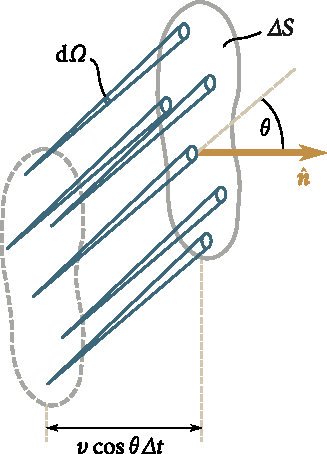
\includegraphics[scale=1.0]{figures/ch_11/fig_11_5.pdf}
		\caption[]{}
		\label{fig:11_5}
	\end{center}
	\vspace{-0.8cm}
\end{figure}

Từ $N$ phân tử chứa trong bình ta tách $\deriv{N_v}$ phân tử có độ lớn vận tốc nằm trong phạm vi từ $v$ đến $v$ đến $v+\deriv{v}$. Trong số các phân tử này sẽ có một số lượng phân tử bằng
\begin{equation}\label{eq:11_18}
	\deriv{N_{v,\theta,\varphi}} = \deriv{N_v} \frac{\deriv{\Omega_{\theta,\varphi}}}{4\pi}
\end{equation}

\noindent
với các hướng chuyển động nằm trong góc khối $\Delta \Omega$ ( xem \fig{11_17}). Trong các phân tử được tách ra bằng cách đó các ơhân tử chứa trong hình trụ xiên với đáy $\Delta S$ và độ cao $(v\cos\theta)\Delta t$ (\fig{11_15}) sẽ bay đến diện tích $\Delta S$ và va chạm vào đó \footnote[1]{$\medskip$ Hình như có thể phản đối lại rằng, một phần các phân tử này trên đường đi tới thành bị va chạm với các phân tử khác, do đó thay đổi hướng chuyển động và không đạt tới diện tích $\Delta S$. Tuy nhiên các va chạm không vi phạm tính chất hỗn loạn của chuyển động các phân tử: sự chuyển một số lượng phân tử nào đó từ một nhóm chuyển động theo hướng tới thành bình vào nhóm chuyển động theo các hướng khác được kèm theo sự chuyển đồng thời cùng một số phân tử từ nhóm khác vào nhóm chuyển động theo hướng tới thành bình. Do đó khi tính số lượng phân tử bay đến thành bình có thể không chú ý tới các va chạm của các phân tử với nhau.} trong thời gian $\Delta t$. Số lượng các phân tử này bằng 
\begin{equation}\label{eq:11_19}
	\deriv{\nu_{v,\theta,\varphi}} = \deriv{N_v} \frac{\deriv{\Omega_{\theta,\varphi}}}{4\pi}\frac{\Delta S (v\cos\theta)\Delta t}{V}
\end{equation}

\noindent
($V$ là thể tích của bình). Để nhận được tổng số va chạm của các phân tử vào diện tích $\Delta S$, cần phải lấy tổng biểu thức \eqn{11_19} theo góc khối $2\pi$ (ứng với các biến đổi của $\theta$ từ $0$ dến $\pi/2$ và các biến đổi của $\varphi$ từ $0$ đến $2\pi$) và theo các vận tốc trong phạm vi từ $0$ đến $\ab{v}{max}$, trong đó $\ab{v}{max}$ là vận tốc lớn nhất mà các phân tử có thể có trong các điều kiện đã cho (xem mục trước).

Ta hãy bắt đầu từ sự lấy tổng theo các hướng. Muốn vậy ta biểu diễn $\deriv{\Omega}$ dưới dạng $\sin \theta\,\deriv{\theta}\,\deriv{\varphi}$ (xem \eqn{11_15}) và tiến hành lấy tích phân biểu thức \eqn{11_19} theo $\theta$ trong phạm vi từ $0$ đến $\pi/2$ và theo $\varphi$ trong phạm vi từ $0$ đến $2\pi$:
\begin{equation*}
	\deriv{\nu_v} = \frac{\deriv{N_v} v \Delta S \Delta t}{4\pi V} \int_{0}^{\pi/2} \cos\theta\sin\theta\,\deriv{\theta} \int_{0}^{2\pi} \deriv{\varphi}.
\end{equation*}

\noindent
Việc lấy tích phân theo $\deriv{\varphi}$ cho $2\pi$, tích phân theo $\deriv{\theta}$ bằng $1/2$. Do đó,
\begin{equation}\label{eq:11_20}
	\deriv{\nu_{v}} = \frac{\deriv{N_v} v \Delta S \Delta t}{4V}.
\end{equation}

\noindent
Biểu thức này cho số va chạm vào diện tích $\Delta S$ trong thời gian $\Delta t$ của các phân tử bay theo các phương bao hàm trong phạm vi của góc khối $2\pi$ và có giá trị của vận tốc từ $v$ đến $v+\deriv{v}$.
Lấy tổng theo các vận tốc sẽ cho tổng số các va chạm của các phân tử vào diện tích $\Delta S$ trong thời gian $\Delta t$: 
\begin{equation}\label{eq:11_21}
	\nu_{\Delta S,\Delta t} = \frac{\Delta S \Delta t}{4V} \int_{0}^{\ab{v}{max}} v\,\deriv{N_v}.
\end{equation}

\noindent
Biểu thức
\begin{equation*}
	\frac{1}{N}\int_{0}^{\ab{v}{max}} v\,\deriv{N_v}
\end{equation*}

\noindent
là giá trị trung bình của độ lớn của vận tốc $v$. Thay tích phân trong \eqn{11_21} bằng tích $N\average{v}$ ta được:
\begin{equation}\label{eq:11_22}
	\nu_{\Delta S,\Delta t} = \frac{\Delta S \Delta t}{4V} N\average{v} = \frac{1}{4}n \average{v}\Delta S \Delta t.
\end{equation}

\noindent

Ở đây $n=N/V$ là số phân tử khi trong một đơn vị thể tích.

Cuối cùng, chia biểu thức \eqn{11_22} cho $\Delta S$ và $\Delta t$ ta tìm được số va chạm của các phân tử khí vào một đơn vị bề mặt thành bình trong một đơn vị thời gian:Nếu giữ nguyên giả thuyết
\begin{equation}\label{eq:11_23}
	\nu = \frac{1}{4} n \average{v}.
\end{equation}

\noindent
Kết quả thu được có ý nghĩa là số va chạm tỷ lệ với số lượng phân tử trong một đơn vị thể tích (``nồng độ`` phân tử) và giá trị trung bình của độ lớn của vận tốc của các phần tử \footnote[1]{$\medskip$ Ta chú ý tới module của vận tốc. Giá trị trung bình của vector vận tốc của các phân tử trong trường hợp chát khí ở trạng thái cân bằng là bằng không.}. Ta thấy rằng đại lượng $\nu$ trong \eqn{11_23} là mật độ dòng phân tử đập vào thành.

Ta hình dung trong chất khí một diện tích đơn vị được tưởng tượng. Nếu chất khí ở trạng thái cân bằng thì qua diện tích này, một số lượng phân tử như nhau về trung bình sẽ bay qua trong một đơn vị thời gian theo mỗi hướng cũng được xác định bằng công thức \eqn{11_23}.

Với sự chính xác đến một hệ số bằng số, ta có thể thu được biểu thức~\eqref{eq:11_23} bằng các lập luận được đơn giản hóa như sau. Ta giả sử rằng các phân tử khi chuyển động chỉ dọc theo ba hướng vuông góc với nhau. Nếu trong bình có chứa $N$  phân tử khí thì tại một thời điểm tùy ý, sẽ có $N/3$ phân tử đó (nghĩa là $N/6$ phân tử) chuyển động dọc theo phương đã cho về phía này, một nửa về phía kia. Do đó sẽ có 1/6 số phân tử chuyển động về hướng mà ta quan tâm (chẳng hạn, theo phương pháp tuyến với yếu tố $\Delta S$ đã cho của thành bình).


\begin{figure}[!htb]
	\begin{center}
		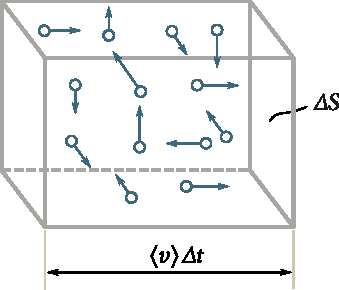
\includegraphics[scale=1.0]{figures/ch_11/fig_11_6.pdf}
		\caption[]{}
		\label{fig:11_6}
	\end{center}
	\vspace{-0.8cm}
\end{figure}
Ngoài ra, ta giả thử rằng mọi phân tử đều chuyển động với cùng vận tốc  $\average{v}$. Khi đó trong thời gian $\Delta t$, tất cả các phân tử chuyển động hướng tới yếu tố thành bình $\Delta S$ được chứa đựng trong thể tích hình trụ với đáy $\Delta S$ và chiều cao $\average{v}\Delta t$ (\fig{11_6}) sẽ bay tới yếu tố thành bình $\Delta S$. Số phân tử này bằng $\Delta\nu=(n/6)\Delta S\average{v}\Delta t$. Một cách tương ứng số va chạm vào một diện tích đơn vị trong một đơn vị thời gian là bằng
\begin{equation}\label{eq:11_24}
	\nu = \frac{1}{6}n\average{v}.
\end{equation}

\noindent


Biểu thức thu được khác với \eqn{11_23} chỉ bởi giá trị của thừa số bằng ($1/6\, \texttt{thay cho}\, 1/4$).

Nếu giữ nguyên giả thuyết về sự chuyển động của các phân tử theo ba hướng vuông góc với nhau nhưng từ bỏ giả thuyết về sự đồng nhất của các vận tốc của các phân tử, thì phải tác ra từ số phân tử trong một đơn vị thể tích, $\deriv{n_v}$ phân tử có vận tốc nằm trong khoảng từ $v$ đến $v+\deriv{v}$. Số lượng phân tử có các vậntốc như thế và bay đến diện tích $\Delta S$ trong thời gian $\Delta t$ sẽ bằng
\begin{equation}\label{eq:11_25}
	\deriv{\nu_v} = \frac{1}{6}v\Delta S \Delta t\,\deriv{n_v}.
\end{equation}

\noindent
Ta thu được tổng số các va chạm bằng cách lấy tích phân biểu thức \eqn{11_25} theo các vận tốc:
\begin{equation*}
	\Delta\nu = \int \deriv{\nu_v} = \frac{1}{6} \Delta S \Delta t \int_{0}^{\ab{v}{max}} v\,\deriv{n_v} = \frac{1}{6}n \average{v}\Delta S \Delta t.
\end{equation*}

\noindent
Cuối cùng, chia $\Delta\nu$ cho $\Delta S$ và $\Delta t$, ta được công thức \eqn{11_24}. Vậy giả thiết về sự đồng nhất của các vận tốc các phân tử không ảnh hưởng đến kết quả thu được đối với số va chạm của các phân tử vào thành bình. Tuy nhiên, như ta thấy ở mục sau, giả thiết này làm thay đổi kết quả của các phép tính áp suất.

\section{Áp suất của chất khí lên thành}\label{sec:11_4}

Các thành của bình đựng khi bị các phân tử oanh kích liên tục. Kết quả là một nguyên tố $\Delta S$ của thành trong một giây được truyền cho một động lượng là bằng lực tác dụng lên $\Delta S$. Tỷ số của lực này với đại lượng $\Delta S$ cho áp suất do chất khí tác dụng lên thành bình. Do các phân tử chuyển động hỗn loạn, áp suất của chất khí tại các phần khác nhau của thành bình là như nhau (dĩ nhiên với điều kiện là chất khí ở trạng thái cân bằng).
\begin{figure}[!htb]
	\begin{center}
		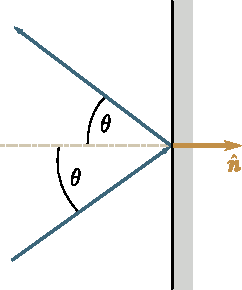
\includegraphics[scale=1.0]{figures/ch_11/fig_11_7.pdf}
		\caption[]{}
		\label{fig:11_7}
	\end{center}
	\vspace{-0.8cm}
\end{figure}

Nếu giả thiết là các phân tử lật lại từ thành theo định luật phản xạ gương ($\ab{\theta}{px} = \ab{\theta}{t}$) và giá trị của vận tốc phân tử không bị biến đổi \footnote[1]{$\medskip$ Thật ra sự tương tác của các phần tử với thành bình mang đặc tính phức tạp hơn (xem phần.~\ref{sec:16_6}) và các giả thiết do ta  đặt ra chỉ đúng về trung bình đối với một số lớn va chạm} thì động lượng do một phân tử truyền cho thành trong một va chạm sẽ bằng $2mv\cos\theta$ (\fig{11_7}; $m$ là khối lượng của phân tử). động lượng này hướng theo pháp tuyến của diện tích. Mỗi phân tử trong $\deriv{\nu_{v,\theta,\varphi}}$ phân tử  (xem \eqn{11_19}) truyền cho thành một động lượng $2mv\cos\theta$, còn tất cả các phân tử này truyền cho thành một động lượng 

\begin{equation*}
	\deriv{K_{v,\theta,\varphi}} = 2mv\cos\theta\,\deriv{\nu_{v,\theta,\varphi}} = \deriv{N_v} \frac{\deriv{\Omega_{\theta,\varphi}}}{4\pi}\frac{2mv^2\cos^2\theta\Delta S\Delta t}{V}.
\end{equation*}

\noindent
(Chúng ta đã sử dụng kí tự $K$ để kí hiệu động lượng hay vì kí tự trước $p$ để tránh sự nhầm lẫn --- kí tự $p$ sẽ tượng trưng cho áp suất sau này)
Ta kấy tổng biểu thức thu được theo các hướng trong phạm vi góc khối $2\pi$ (ứng với các biến thiên của $\theta$ từ $0$ đến $\pi/2$ và các biến thiên của $\varphi$ từ $0$ đến $2\pi$). Kết quả là ta thu được một động lượng được truyền bởi các phần tử với vận tốc có giá trị từ $v$ đến $v+\deriv{v}$:

\begin{equation*}
	\deriv{K_v} = \deriv{N_v} \frac{2mv^2\Delta S\Delta t}{4\pi V} \int_{0}^{\pi/2}\cos^2\theta\sin\theta\,\deriv{\theta} \int_{0}^{2\pi}\deriv{\varphi}
\end{equation*}

\noindent
(ta đã thế biểu thức \eqn{11_15} đối với $\deriv{\omega}4$). Lấy tích phân theo $\deriv{\varphi}$ ta được $2\pi$, tích phân theo $\deriv{\theta}$ bằng $1/3$. Do đó
\begin{equation*}
	\deriv{K_v} = \deriv{N_v} \frac{mv^2\Delta t}{3V}.
\end{equation*}

\noindent
Lấy tích phân biểu thức này theo các vận tốc từ $0$ đến $\ab{v}{max}$ ta thu được động lượng toàn phần truyền cho diện tích $\Delta S$ trong thời gian $\Delta t$:
\begin{equation}\label{eq:11_26}
	\Delta K = \frac{m\Delta S\Delta t}{3V} \int_{0}^{\ab{v}{max}} v^2\,\deriv{N_v}.
\end{equation}

Biểu thức
\begin{equation*}
	\frac{1}{N}\int_{0}^{\ab{v}{max}} v^2\,\deriv{N_v}
\end{equation*}

\noindent
là giá trị trung bình của bình phương vận tốc các phân tử. Thay tích phân trong \eqn{11_26} bằng tích $N\average{v^2}$, ta thu được 
\begin{equation*}
	\Delta K = \frac{m\Delta S\Delta t}{3V} N \average{v^2} = \frac{1}{3} nm \average{v^2} \Delta S\Delta t
\end{equation*}

\noindent
($n=N/V$ là số phân tử trong một đơn vị thể tích). Cuối cùng, chia biểu thức này cho $\Delta S$ và $\Delta t$ ta thu được áp suất khí lên thành bình:
\begin{equation}\label{eq:11_27}
	p = \frac{1}{3} nm \average{v^2} = \frac{2}{3} n \frac{m\average{v^2}}{2}.
\end{equation}

Khối lượng của tất cả các phần tử theo giả thiết là như nhau. Do đó có thể đưa nó vào trong dấu trung bình. Kết quả là biểu thức \eqn{11_27} có dạng
\begin{equation}\label{eq:11_28}
	p = \frac{2}{3} n \average{\frac{mv^2}{2}} = \frac{2}{3}n\average{\ab{\varepsilon}{tr}}
\end{equation}

\noindent
trong đó $\average{\ab{\varepsilon}{tr}}$ là giá trị trung bình của động năng chuyển động tịnh tiến của các phần tử.

Ta thu được biểu thức đối với áp suất, xuất phát từ các quan niệm đã được đơn giản hóa dẫn ta tới công thức \eqn{11_24}. Theo các quan niệm này khi va chạm mỗi phần tử truyền cho thành bình một động lượng $2m\average{v}$. Nhân động lượng này với số va chạm (xem \eqn{11_24}) ta thu được động lượng truyền cho diện tích đơn vị trong một đơn vị thời gian, nghĩa là áp suất. Vậy ta thu được công thức 
\begin{equation}\label{eq:11_29}
	p = \frac{1}{6} n \average{v} \times 2m\average{v} = \frac{1}{3}nm\average{v}^2.
\end{equation}

\noindent
Công thức này khác \eqn{11_27} ở chỗ thay cho bình phương trung bình của vận tốc $\average{v^2}$ là bình phương của vận tốc trung bình $\average{v}^2$. Sau này (xem~\ref{sec:11_5}) ta thấy rõ là hai đại lượng này khác nhau, nghĩa là $\average{v^2}\neq\average{v}^2$.

Nếu tính cẩn thận hơn thì cần nhân số phân tử được xác định bằng công thức \eqn{11_25} với $2mv$ và sau đó tiến hành lấy tổng theo mọi $v$. Kết quả là ta thu được động lượng truyền cho diện tích $\Delta S$ trong thời gian $\Delta t$:
\begin{align*}
	\Delta K &= \int_{0}^{\ab{v}{max}} \frac{1}{6}\,\deriv{n_v}\Delta S\Delta t \times 2mv = \frac{1}{3}m \Delta S\Delta t \int_{0}^{\ab{v}{max}} v^2\,\deriv{n_v}\\
	&= \frac{1}{3}nm\average{v^2} \Delta S\Delta t.
\end{align*}

\noindent
Chia biểu thức này cho $\Delta S$ và $\Delta t$, ta thu được công thức \eqn{11_27} đối với áp suất. Vậy xuất phát từ một quan niệm đã được đơn giản háo về chuyển động của các phân tử dọc theo ba phương vuông góc với nhau, ta đã thu được biểu thức chính xác cho áp suất. Điều này được giải thích là sự đơn giản hóa đã chỉ ra, mmột mặt, dẫn tới sự hạ thấp số va chạm của các phân tử vào thành ($n\average{v}/6$ thay cho $n\average{v}/4$, xem ~\eqref{eq:11_23} và ~\eqref{eq:11_24}), còn mặt khác dẫn tới sự nâng cao động lượng truyền cho thành trong mỗi va chạm. Với kết luận được đơn giản hóa ta đã nhận thấy rằng trong mỗi va chạm, một động lượng bằng $2mv$ được truyền cho thành. Thực ra chính giá trị của động lượng truyền cho thành phụ thuộc vào góc $\theta$, vì vậy động lượng trung bình được truyền trong một va chạm là bằng $4mv/3$. Rốt cuộc, cả hai sự không chính xác bù trừ lẫn cho nhau và mặc cho sự đơn giản hóa cách nghiên cứu, người ta vẫn thu được biểu thức chính xác cho áp suất.

\section{Năng lượng trung bình của các phân tử}\label{sec:11_5}

Ta viết liền nhau biểu thức \eqn{11_28} thu được trong mục trước cho áp suất và phương trình trạng thái khí lý tưởng~\eqref{eq:10_21}:
\begin{equation*}
	p = \frac{2}{3}n\average{\ab{\varepsilon}{tr}},\quad p = nkT.
\end{equation*}

\noindent
Từ việc so sánh các biểu thức này suy ra rằng
\begin{equation}\label{eq:11_30}
	\average{\ab{\varepsilon}{tr}} = \frac{3}{2}kT.
\end{equation}
%\average{\ab{\varepsilon}{tt}} (trong bản scan) đã đổi thành \average{\ab{\varepsilon}{tr}} cho giống sách gốc, cũng tránh nhầm lẫn với những đoạn mã code trong đây.
\noindent
Vậy ta đã đi tới một kết luận quan trọng: \textbf{nhiệt độ tuyệt đối là một đại lượng tỷ lệ với năng lượng trung bình của chuyển động tịnh tiến của các phân tử.} Các phân tử khí chỉ chuyển động tịnh tiến. Đối với các chất lỏng và các chất rắn năng lượng trung bình của các phân tử tỷ lệ với nhiệt độ tuyệt đối chỉ trong trường hợp khi chuyển động của các phân tử có đặc tính cổ điển. Trong lĩnh vực lượng tử sự tỷ lệ giữa năng lượng trung bình của các phân tử và nhiệt độ tuyệt đối không được tuân thủ.

Biểu thức~\eqref{eq:11_30} đáng chú ý ở chỗ là năng lượng trung bình chỉ phụ thuộc vào nhiệt độ mà không phụ thuộc vào khối lượng của phân tử.

Vì $\average{\ab{\varepsilon}{tr}}=\average{mv^2/2}=(m/2)\average{v^2}$ nên từ \eqn{11_30} suy ra rằng 


\begin{equation}\label{eq:11_31}
	\average{v^2} = \frac{3kT}{2m}.
\end{equation}

\noindent

Biểu diễn $\average{v^2}$ dưới dạng tổng các bình phương của các thành phần vận tốc, có thể viết:
\begin{equation}
   \average{v^2} = \average{v_x^2} + \average{v_y^2} + \average{v_x^2}.
\end{equation}
Do sự tương đương của tất cả các hướng chuyển động nên đẳng thức sau được nghiệm đúng:
\begin{equation*}
	\average{v_x^2} = \average{v_y^2} = \average{v_z^2}.
\end{equation*}

\noindent
Để ý tới điều này ta tìm được
\begin{equation}\label{eq:11_32}
	\average{v_x^2} = \frac{1}{3}\average{v^2} = \frac{kT}{m}.
\end{equation}
Công thức~\eqref{eq:11_30} xác định năng lượng chỉ của chuyển động tịnh tiến của phân tử. Tuy vậy cùng với chuyển động tịnh tiến cũng có thể có sự quay của phân tử và dao động của các nguyên tử tham gia vào thành phần của phân tử. Cả hai dạng chuyển động này được gắn với một dự trữ năng lượng nào đó, mà giả thuyết về sự phân bố năng lượng theo bậc tự do của phân tử được thiết lập bằng vật lý thống kê cho phép xác định dự trữ năng lượng này.

\textit{Số bậc tự do của một hệ cơ học là số lượng đại lượng độc lập mà nhờ chúng có thể xác lập vị trí của hệ}. Như vậy vị trí của một chất điểm trong không gian hoàn toàn được xác định bằng việc cho các giá trị của ba tọa độ của nó (chẳng hạn, các tọa độ Descartes $x, y, z$ hoặc các tọa độ cầu $r, \theta, \varphi$, v.v$\ldots$). Căn cứ vào điều này một chất điểm có ba bậc tự do.

\begin{figure}[!htb]
	\begin{center}
		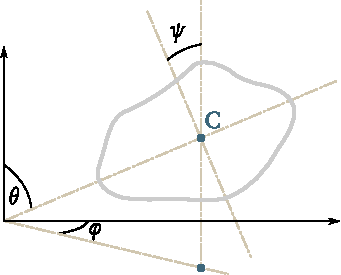
\includegraphics[scale=1.0]{figures/ch_11/fig_11_8.pdf}
		\caption[]{}
		\label{fig:11_8}
	\end{center}
	\vspace{-0.8cm}
\end{figure}

Có thể xác định vị trí của một vật rắn tuyệt đối bằng cách cho ba tọa độ của khối tâm của nó $(x, y, z)$, hai góc $\theta$ và $\varphi$ chỉ hướng của một trục nào đó gắn với vật và đi qua khối tâm của nó (\fig{11_8}), và cuối cùng, góc $\psi$ xác định hướng của một trục thứ hai gắn với vật, vuông góc với trục thứ nhất. Vậy một vật rắn tuyệt đối có sáu bậc tự do. Sự biến đổi các tọa độ của khối tâm khi các góc $\theta$, $\varphi$ và $\psi$ không biến đổi được gây bởi chuyển động tịnh tiến của vật rắn. Do đó các bậc tự do tương ứng được gọi là các \textbf{bậc tự do tịnh tiến}. Sự biến đổi của một góc bất kỳ trong các góc $\theta$, $\varphi$, $\psi$ khi vị trí của khối tâm không thay đổi sẽ được gây ra bởi sự quay của vật, cho nên các bậc tự do tương ứng được gọi là các \textbf{bậc tự do quay}. Do đó trong sáu bậc tự do của vật rắn tuyệt đối, thì có  ba là các bậc tự do tịnh tiến và có ba là các bậc tự do quay.

Hệ gồm $N$ chất điểm mà giữa chúng không có các liên kết rắn sẽ có $3N$ bậc tự do (vị trí của mỗi điểm trong $N$ điểm phải được quy định bằng ba tọa độ). Một liên kết rắn bất kỳ xác lập vị trí tương hỗ không thay đổi của hai điểm làm giảm số bậc tự do một đơn vị. Chẳng hạn, nếu hệ gồm hai chất điểm mà khoảng cách $l$ giữa chúng là không đổi (\fig{11_9}) thì số bậc tự do của hệ là bằng năm. Thực vậy, trong trường hợp này giữa các tọa độ của các điểm có hệ thức:
\begin{equation}\label{eq:11_33}
	(x_2 - x_1)^2 + (y_2 - y_1)^2 + (z_2 - z_1)^2 = l^2
\end{equation}

\noindent
do đó các tọa độ sẽ không độc lập với nhau: cho năm tọa độ bất kỳ là đủ, còn tọa độ thứ sáu được xác định bằng điều kiện~\eqref{eq:11_33}. Để phân loại năm bậc tự do này ta chú ý rằng có thể xác định vị trí của hệ gồm hai chất điểm liên kết rắn bằng cách sau: cho ba tọa độ của khối tâm hệ (\fig{11_10}) và hai góc $\theta$ và $\varphi$ xác định hướng của một trục của hệ trong không gian (nghĩa là đường thẳng đi qua hai điểm). Từ đó suy ra bằng ba bậc tự do là các bậc tự do tịnh tiến, còn hai bậc tự do là các bậc tự do quay. Các bậc tự do quay ứng với phép quay xung quanh hai trục vuông góc với nhau $O'O'$ và $O''O''$, vuông góc với trục $OO$ của hệ (\fig{11_11}). Phép quay xung quanh trục $OO$ đối với các chất điểm là không có ý nghĩa.

\begin{figure}[!htb]
	\begin{minipage}[t]{0.5\linewidth}
		\begin{center}
			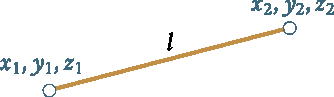
\includegraphics[scale=1.0]{figures/ch_11/fig_11_9.pdf}
			\caption[]{}
			\label{fig:11_9}
		\end{center}
	\end{minipage}
	\hspace{-0.05cm}
	\begin{minipage}[t]{0.5\linewidth}
		\begin{center}
			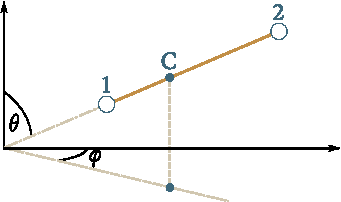
\includegraphics[scale=1.0]{figures/ch_11/fig_11_10.pdf}
			\caption[]{}
			\label{fig:11_10}
		\end{center}
	\end{minipage}
%	\vspace{-0.4cm}
\end{figure}

\begin{figure}[!htb]
	\begin{minipage}[t]{0.5\linewidth}
		\begin{center}
			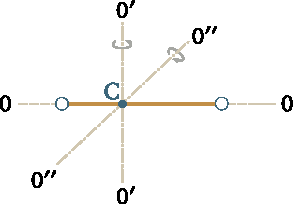
\includegraphics[scale=1.0]{figures/ch_11/fig_11_11.pdf}
			\caption[]{}
			\label{fig:11_11}
		\end{center}
	\end{minipage}
	\hspace{-0.05cm}
	\begin{minipage}[t]{0.5\linewidth}
		\begin{center}
			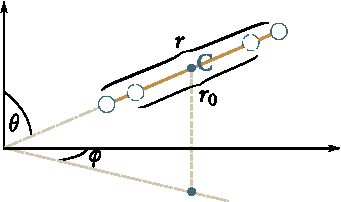
\includegraphics[scale=1.0]{figures/ch_11/fig_11_12.pdf}
			\caption[]{}
			\label{fig:11_12}
		\end{center}
	\end{minipage}
	\vspace{-0.4cm}
\end{figure}


Nếu hai chất điểm liên kết với nhau không bằng liên kết rắn mà bằng liên kết đàn hồi (nghĩa là sao cho mỗi sự biến đổi khoảng cách cân bằng $r_0$ giữa các điểm kéo theo sự xuất hiện các lực có xu hướng thiết lập lại khoảng cách ban đầu giữa các điểm) thì số bậc tự do sẽ bằng sáu. Trong trường hợp này có thể xác định vị trí của hệ bằng cách cho ba tọa độ của khối tâm (\fig{11_12}), hai góc $\theta$, $\varphi$ và khoảng cách $r$ giữa các điểm. NHững thay đổi của $r$ ứng với các dao động trong hệ, vì vậy người ta gọi bậc tự do này là \textbf{bậc tự do dao động}.
Vậy hệ được xét có ba bậc tự do tịnh tiến, hai bậc tự do quay và một bậc tự do dao động.

Ta xét hệ gồm $N$ chất điểm liên kết đàn hồi với nhau. Một hệ như vậy $3N$ bậc tự do. Có một cấu hình cân bằng của các điểm ứng với cực tiểu của thế năng của hệ. Cấu hình cân bằng được đặc trưng bằng khoảng cách tương hỗ được xác định hoàn toàn giữa các điểm. Nếu đưa các điểm ra khỏi các vị trí ứng với một cấu hình cân bằng thì các dao động xuất hiện trong hệ. Có thể xác định vị trí của hệ bằng cách cho vị trí của cấu hình cân bằng và các đại lượng đặc trưng sự dịch chuyển của các điểm khỏi các vị trí cân bằng. Các đại lượng này ứng với các bậc tự do dao động. 

Vị trí của cấu hình cân bằng cũng như vị trí của vật rắn tuyệt đối được xác định bằng sáu đại lượng mà ứng với chúng là ba bậc tự do tịnh tiến và ba bậc tự do quay. Vậy số lượng bậc tự do quay bằng $3N-6$\footnote[1]{$\medskip$ Người ta cho rằng các vị trí cân bằng của các điểm không nằm trên một đường thẳng. Trong trường hợp ngược lại các bậc tự do quay sẽ chỉ là hai, còn các bậc tự do dao động là $3N-5$. Ta đã gặp trường hợp như vậy khi xét hệ gồm hai chất điểm.}.

Từ các thí nghiệm về đo nhiệt dung của các chất khí suy ra rằng khi xác định số bậc tự do của phân tử cần coi các nguyên tử như các chất điểm. Do đó, cần gán cho một phân tử đơn nguyên tử ba bậc tự do tịnh tiến, tùy thuộc vào đặc tính của liên kết giữa các nguyên tử, cần gán cho một phân tử lưỡng nguyên tử hoặc ba bậc tự do tịnh tiến và hai bậc tự do quay (với liên kết rắn) hoặc ngoài năm bậc tự do này còn thêm một bậc tự do dao động (với liên kết đàn hồi), gán cho một phân tử tam nguyên tử với liên kết rắn - ba bậc tự do tịnh tiến và ba bậc tự do quay, v.v\ldots

Ta chú ý rằng một phân tử dù có bao nhiêu bậc tự do đi nữa thì ba trong số đó là các bậc tự do tịnh tiến. Vì không có một bậc tự do tịnh tiến nào của phân tử có ưu thế hơn các bậc tự do tịnh tiến còn lại nên về trung bình phải quy cho mỗi bậc tự do một năng lượng như nhau bằng một phần ba giá trị \eqn{11_30}, nghĩa là $\frac{1}{2}kT$.

Trong vật lý thống kê cổ điển người ta đưa ra \footnote[2]{$\medskip$ Kết luận này ra ngoài phạm vi của giáo trình vật lý đại cương.} \textbf{định luật phân bố đều}, theo định luật này \textit{về trung bình phải quy cho mỗi bậc tự do của phân tử một động năng như nhau bằng $\frac{1}{2}kT$.}

Theo định luật phân bố đều, giá trị trung bình của năng lượng của một phân tử $\average{\varepsilon}$ (ở cùng một nhiệt độ) sẽ càng lớn nếu phân tử càng phức tạp, nghũa là nếu nó có các bậc tự do dao động phải có dung lượng năng lượng lớn gấp đôi so với bậc tự do tịnh tiến và quay. Điều này được giải thích là chuyển động tịnh tiến và chuyển động quay của phân tử liên hệ với sự có mặt chỉ của động năng, trong khi mà chuyển động dao động liên hệ với sự có mặt của cả động năng lẫn thế năng, thêm vào đó đôi với dao động tử điều hòa, giá trị trung bình của động năng và thế năng là như nhau. Do đó, về trung bình, hai nửa của $kT$ - một dưới dạng động năng và một dưới dạng thế năng - phải ứng với mỗi bậc tự do dao động.

Vậy năng lượng trung bình của một phân tử phải bằng

\begin{equation}\label{eq:11_34}
	\average{\varepsilon} = \frac{i}{2}kT
\end{equation}

\noindent

trong đó $i$ là tổng của số bậc tự do tịnh tiến ($\ab{n}{tr}$), số bậc tự do quay ($\ab{n}{rot}$) và hai lần số bậc tự do dao động của phân tử ($\ab{n}{vib}$):
\vspace{5pt}
\begin{equation}\label{eq:11_35}
	i = \ab{n}{tr} + \ab{n}{rot} + 2\ab{n}{vib}.
\end{equation}
% trong bản scan thì hay vì tr trong thì họ dùng tt cho tịnh tiến, q cho quay, dđ cho dao động, tuy nhiên để tránh nhầm lẫn mình không dịch theo như vậy.
\noindent
For molecules with a rigid bond between their atoms, $i$ coincides with the number of degrees of freedom of a molecule.
Đối với các phân tử có liên kết rắn giữa các nguyên tử thì trùng với số bậc tự do của phân tử.

Các phân tử khí lý tưởng không tương tác với nhau. Do đó có thể tìm được nội năng của một mol khí lý tưởng bằng cách nhân số Avogardo với năng lượng trung bình của một phân tử:
\begin{equation}\label{eq:11_36}
	\ab{U}{m} = \ab{N}{A}\average{\varepsilon} = \frac{i}{2}\ab{N}{A} kT = \frac{i}{2}RT.
\end{equation}

\noindent
So sánh biểu thức này với \eqn{10_28} ta được 
\begin{equation}\label{eq:11_37}
	C_V = \frac{i}{2}R.
\end{equation}

\noindent
Chú ý tới công thức \eqn{10_33}, ta tìm được:
\begin{equation}\label{eq:11_38}
	C_p = \left(\frac{i+2}{2}\right) R.
\end{equation}

\noindent
Do đó,
\begin{equation}\label{eq:11_39}
	\gamma = \frac{C_p}{C_V} = \frac{i+2}{i}.
\end{equation}

\noindent
Vậy đại lượng $\gamma$ được xác định bằng số và bằng tính chất của các bậc tự do của phân tử.

Trong bảng~\ref{table:11_1} người ta đưa vào các giá trị $C_V$, $C_p$ và $\gamma$ thu được đối với các phân tử khác nhau theo các công thức~\eqref{eq:11_37}, \eqref{eq:11_38}, và~\eqref{eq:11_39}. Trong bảng~\ref{table:11_2} ta so sánh các kết quả của lý thuyết với các dữ kiện thực nghiệm. Các giá trị lý thuyết sẽ thu được (trừ một trường hợp đã chỉ ra trong ghi chú ở bảng) với giả thuyết là các phân tử là rắn; các giá trị thực nghiệm sẽ thu được đối với các nhiệt độ gần nhiệt độ phòng.
\begin{table}[!b]
	\renewcommand{\arraystretch}{1.2}
	\caption{ }
	\vspace{-0.6cm}
	\label{table:11_1}
	\begin{center}\resizebox{0.82\linewidth}{!}{
			\begin{tabular}{l p{1.59cm} ccccccc}
				\toprule[1pt]
				\multirow{2}{*}{\textbf{Phân tử}} & \textbf{Tính chất của liên kết giữa các nguyên tử} & \multirow{2}{*}{$\ab{n}{tr}$} & \multirow{2}{*}{$\ab{n}{rot}$} & \multirow{2}{*}{$\ab{n}{vib}$} & \multirow{2}{*}{$i$} & \multirow{2}{*}{$C_V$} & \multirow{2}{*}{$C_p$} & \multirow{2}{*}{$\gamma$}\\
				\midrule[0.5pt]\midrule[0.5pt]
				Đơn nguyển tử & --- & $3$ & --- & --- & $3$ & $\frac{3}{2}R$ & $\frac{5}{2}R$ & $1.67$\\
				Lưỡng nguyên tử & Rắn & $3$ & $2$ & --- & $5$ & $\frac{5}{2}R$ & $\frac{7}{2}R$ & $1.40$\\
				Lưỡng nguyên tử & Đàn hồi & $3$ & $2$ & $1$ & $7$ & $\frac{7}{2}R$ & $\frac{9}{2}R$ & $1.29$\\
				$\geqslant 3$ nguyên tử & Rắn & $3$ & $3$ & --- & $6$ & $\frac{6}{2}R$ & $\frac{8}{2}R$ & $1.33$\\
				\bottomrule[1pt]
			\end{tabular}
	}\end{center}
\end{table}

\begin{table}[!b]
	\renewcommand{\arraystretch}{1.2}
	\caption{ }
	\vspace{-0.6cm}
	\label{table:11_2}
	\begin{center}\resizebox{0.98\linewidth}{!}{
			\begin{threeparttable}[b]
			\begin{tabular}{lccccccc}
				\toprule[1pt]
				\multirow{2}{*}{\textbf{Chất khí}} & \multirow{2}{2.3cm}{\textbf{Số nguyên tử trong một phân tử}} & \multicolumn{2}{c}{$C_V\times\num{e-3}$} &
				\multicolumn{2}{c}{$C_p\times\num{e-3}$} & \multicolumn{2}{c}{$\gamma$} \\
				& & Lý thuyết. & Thực nghiệm. & Lý thuyết. & Thực nghiệm. & Lý thuyết. & Thực nghiệm.\\
				\midrule[0.5pt]\midrule[0.5pt]
				Helium (He)&$1$&$12.5$&$12.5$&$20.8$&$20.9$&$1.67$&$1.67$\\
				Oxygen (\ce{O2})&$2$&$20.8$&$20.9$&$29.1$&$28.9$&$1.40$&$1.40$\\
				Carbon monoxide (CO)&$2$&$20.8$&$21.0$&$29.1$&$29.3$&$1.40$&$1.40$\\
				Hơi nước (\ce{H2O})&$3$&$25.0$&$27.8$&$33.2$&$36.2$&$1.33$&$1.31$\\
				& & $33.2$\tnote{${\dagger}$} & & $41.5$\tnote{${\dagger}$} & & $1.25$\tnote{${\dagger}$} & \\
				\bottomrule[1pt]
			\end{tabular}
		\begin{tablenotes}
			\item [${\dagger}$] Đối với $i=8$, nghĩa là với giả thiết rằng có một bậc tự do dao động phụ
		\end{tablenotes}
	\end{threeparttable}
	}\end{center}
\end{table}

Hình như, từ bảng~\ref{table:11_2} suy ra rằng sự phù hợp giữa lý thuyết và thực nghiệm trong mọi trường hợp đối với các phân tử đơn và lưỡng nguyên tử là hoàn toàn được thõa mãn. Tuy nhiên, trong thực tế điều này lại không như vậy, Theo lý thuyết nà ta đã xét, các nhiệt dung của các chất thải phải là bội nguyên của $R/2$ hoặc số bậc tự do có thể chỉ là một số nguyên. Do đó ngay cả các độ lệch nhỏ $C_V$ và $C_P$ khỏi các giá trị, bội của $R/2$ cũng đóng vai trò có tính nguyên tắc. Như đã thấy trong bảng,hơn nữa, người ta đã thừa biết các độ lệch như vậy vượt quá các sai số khả dĩ của các phép đo đã xảy ra.

\begin{figure}[!htb]
	\begin{center}
		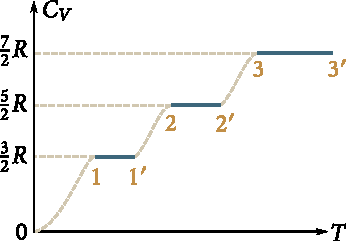
\includegraphics[scale=1.0]{figures/ch_11/fig_11_13.pdf}
		\caption[]{}
		\label{fig:11_13}
	\end{center}
	\vspace{-0.8cm}
\end{figure}

Các sự không phù hợp giữa lý thuyết và thực nghiệm trở nên đặc biệt lạ lùng nếu ta để ý tới sự phụ thuộc vào nhiệt độ của nhiệt dung. Trên hình~\ref{fig:11_13} người ta biểu diễn đường cong về sự phụ thuộc của nhiệt dung của một kilomole $C_V$ vào nhiệt độ thu được bằng thực nghiệm đối với hydro. Theo lý thuyết, nhiệt dung không bị phụ thuộc vào nhiệt độ. Từ hình vẽ rõ ràng điều này chỉ đúng trong phạm vi của các khoảng nhiệt độ riêng biệt, hơn nữa trong các khoảng khác nhau nhiệt dung có các giá trị ứng với số bậc tự do khác nhau của phân tử. Vậy trên $1$-$1'$ thì $C_V=\frac{3}{2}R$. Điều này có nghĩa là phân tử thể hiện như một hệ chỉ có các bậc tự do tịnh tiến. Trên phần $2$-$2'$ thì $C_V=\frac{5}{2}R$. Do đó với các nhiệt độ ứng với phần này. ở một phân tử, ngoài ba bậc tự do tịnh tiến được xuất hiện ở các nhiệt độ thấp hơn còn thêm hai bậc tự do quay. Cuối cùng, ở các nhiệt độ đủ lớn $C_V=\frac{7}{2}R$điều này xác nhận về sự có mặt của các dao động của phân tử ở các nhiệt độ này. Trong các khoảng giữa các khoảng chỉ ra, nhiệt dung tăng đơn điệu với nhiệt độ, nghĩa là như là ứng với một số bậc tự do biến đổi không nguyên. 

Vậy số bậc tự do của phân tử xuất hiện trong nhiệt dung là phụ thuộc vào nhiệt độ. Ở các nhiệt độ thấp người ta chỉ quan sát được sự chuyển động tịnh tiến của phân tử. Ở các nhiệt độ cao hơn, cùng với chuyển động tịnh tiến người ta cũng quan sát được sự quay của các phân tử. Và cuối cùng, ở các nhiệt độ cao hơn, cùng với chuyển động tịnh tiến người ta cũng quan sát được sự quay của các phân tử. Và cuối cùng, ở các nhiệt độ cao hơn nữa các dao động của các phân tử cũng được bổ sung vào hai dạng chuyển động đầu tiên. Khi đó, như suy ra từ tiến trình đơn điệu của đường con nhiệt dung, tất cả các phân tử không bị lôi cuốn ngay vào chuyển động quay và sau đó vào chuyển động dao động. Chẳng hạn, lúc đầu sự quay bắt đầu được quan sát chỉ ở một phần nhỏ các phân tử. Phần này sẽ tăng với sự tăng nhiệt độ và rốt cuộc khi đạt tới một nhiệt độ xác định, thì tất cả các phân tử thực tế sẽ bị lôi cuốn vào chuyển động quay. Quá trình tương tự sẽ xảy ra cả đối với chuyển động dao động của các phân tử.

Cơ học lượng tử sẽ giải thích về hành trạng như vậycủa nhiệt dung. Như lý thuyết lượng tử đã chứng minh, năng lượng của các chuyển động quay và dao động của các phân tử bị lượng tử hóa. Điều này có nghĩa là năng lượng quay và năng lượng dao động của phân tử cps thế có không phải những giá trị bất kỳ mà chỉ những giá trị gián (nghĩa là những giá trị riêng biệt khác nhau một đại lượng hữu hạn). Do đó năng lượng liên hệ với các dạng chuyển động quay có thể chỉ bị biến đổi bằng những bước nhảy. Đối với năng lượng chuyển động tịnh tiến sẽ không tồn tại một sự ràng buộc như vậy.

Các khoảng giữa các giá trị năng lượng cho phép riêng biệt (hoặc như thường nói, giữa các mức năng lượng) đối với sự dao động được ước chừng lớn hơn đối với sự quay. Sơ đồ được đơn giản hóa \footnote[1]{$\medskip$ Trong thực thế các khoảng cách giữa các mức quay là không như nhau. Tuy vậy, điều này không quan trọng đối với vấn đề đang xét.} của các phân mức quay và dao động của một phân tử lưỡng nguyên tử cho trên \fig{11_14}.
 
\begin{figure}[!htb]
	\begin{center}
		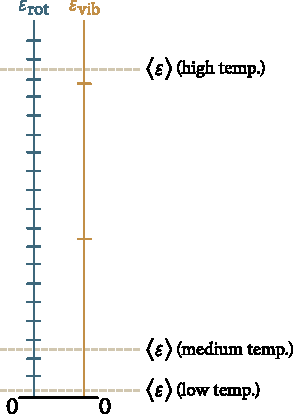
\includegraphics[scale=1.0]{figures/ch_11/fig_11_14.pdf}
		\caption[]{}
		\label{fig:11_14}
	\end{center}
	\vspace{-0.8cm}
\end{figure}

Trong Sec.~\ref{sec:11_2} ta đã nhận xét rằng các vận tốc của các phân tử chủ yếu tụ lại gần một giá trị có xác suất lớn nhất nào đó. Một các tương ứng, phần trội hơn của các phân tử sẽ có các năng lượng gần với giá trị trung bình $\average{\varepsilon}$ và chỉ một phần nhỏ các phân tử có năng lượng vượt quá $\average{\varepsilon}$ rất nhiều. Dop đó để một phần đáng kể các phân tử bị lôi cuốn vào chuyển động quay và chuyển động dao động thì năng lượng trung bìnhcủa chúng phải đủ lớn so với khoảng cách giữa các mức năng lượng tương ứng cho phép.

Ta hãy lấy nhiệt độ thấp tới mức là năng lượng trung bình $\average{\varepsilon}$ của phân tử nhỏ hơn giá trị cho phép đầu tiên của năng lượng chuyển động quay rất nhiều (xem đường thẳng chấm chấm phía dưới hình \fig{11_14}). Khi đó chỉ có một phần không đáng kể của tất cả các phân tử bị lôi cuốn vào chuyển động quay, cho nên thực tế các phân tử khí sẽ chỉ chuyển động tịnh tiến. Những sự thay đổi nhỏ của nhiệt độ sẽ dẫn tới các biến đổi chỉ của năng lượng chuyển động tịnh tiến phù hợp với nhiệt dung của chát khí bằng $3R/2$ (xem phần $1$-$1'$ trên đường cong biểu diễn trên hình \fig{11_13}).

Sự tăng nhiệt độ sẽ kèm theo sự tăng $\average{\varepsilon}$, do đó một phần rất lớn các phân tử bị lôi cuốn vào chuyển động quay. Phần đường cong $1'$-$2$ trên \fig{11_13} ứng với quá trình này.



Sau khi tất cả các phân tử bị lôi cuốn vào chuyển động quay thì phần nằm ngang $2$-$2'$ được bắt đầu. Ở các nhiệt độ ứng với phần này, $\average{\varepsilon}$ còn quá nhỏ so với khoảng cách giữa các mức năng lượng dao động cho phép, do đó trên thực tế sẽ không có các dao động của các phân tử. Với sự tăng nhiệt độ, các phân tử bắt đầu bị lôi cuốn vào chuyển động dao đônbjg với số lượng rất lớn ứng với phần chuyển tiếp $2'$-$3$ trên đường cong nhiệt dung. Cuối cùng, ở nhiệt độ đủ cao tất cả các phân tử hầu như bị lôi cuốn vào chuyển động dao động ứng với nhiệt dung bằng $7R/2$.

Vậy lý thuyết cổ điển về nhiệt dung chỉ là gần đúng đối với các khoảng nhiệt độ riêng biệt, thêm vào đó số bậc tự do của phân tử sẽ tương ứng với từng khoảng.



\section{Phân bố Maxwell}\label{sec:11_6}

Để giải thích cách có thể mô tả định lượng sự phân bố các phân tử theo các giá trị vận tốc ta sử dụng thủ thuật sau. Ta lấy trong không gian tưởng tượng mà ta sẽ gọi là không gian $v$ (không gian các vận tốc) các trục tọa độ vuông góc, theo đó ta bắt đầu đặt các giá trị $v_x$, $v_y$ và $v_z$ của các phân tử riêng rẽ (ta chú ý đến các thành phần vận tốc theo các trục $x$, $y$ và $z$ được lấy trong không gian thông thường). Khi đó một điểm trong không gian này sẽ ứng với vận tốc của mỗi phần tử. Do các va chạm, các vị trí của các điểm sẽ bị biến đổi liên tục nhưng mật độ của chúng tại mỗi vị trí sẽ vẫn không thay đổi (ta nhớ rằng đang xét trạng thái cân bằng của chất khí).


Do sự bình đẳng của tất cả hướng chuyển động, vị trí của các điểm đối với gốc tọa độ sẽ có đối xứng cầu. Do đó mật độ các điểm trong không gian $v$ có thể phụ thuộc chỉ vào module của vận tốc $v$ (hoặc vào $v^2$). Ta kí hiệu mật độ này bằng $Nf(v)$ ($N$ là tổng số phân tử trong khối lượng khí đã cho). Khi đó số lượng phân tử có các thành phần của vận tốc nằm trong phạm vi từ $v_x$ đến $v_x+\deriv{v_x}$, từ $v_y$ đến $v_y+\deriv{v_y}$ và từ $v_z$ đến $v_z+\deriv{v_z}$ có thể biểu diễn dưới dạng

\begin{equation}\label{eq:11_40}
	\deriv{N_{v_x, v_y, v_z}} = Nf(v)\,\deriv{v_x}\,\deriv{v_y}\,\deriv{v_z}
\end{equation}

\noindent

(tích $\deriv{v_x}\,\deriv{v_y}\,\deriv{v_z}$ cho ta yếu tố thể tích trong không gian $v$).

\begin{figure}[!htb]
	\begin{center}
		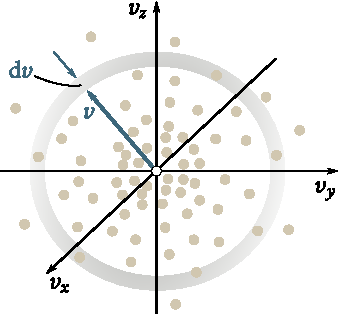
\includegraphics[scale=1.0]{figures/ch_11/fig_11_15.pdf}
		\caption[]{}
		\label{fig:11_15}
	\end{center}
	\vspace{-0.8cm}
\end{figure}

Các điểm biểu diễn vận tốc có độ lớn nằm trong phạm vi từ $v$ đến $v+\deriv{v}$ sẽ rơi vào miền nằm giữa các quả cầu có bán kính $v$ và $v+\deriv{v}$ (\fig{11_15}). Thể tích của miền này bằng $4\pi v^2\,\deriv{v}$. Do đó số điểm ở trong miền này được xác định bằng biểu thức

\begin{equation}\label{eq:11_41}
	\deriv{N_v} = Nf(v) 4\pi v\,\deriv{v}.
\end{equation}

\noindent
Biểu thức này cho số phân tử có giá trị của các vận tốc nằm trong khoảng từ $v$ đến $v+\deriv{v}$. Chia nó cho $N$, ta được xác suất $\deriv{P_v}$ để vận tốc của phân tử rơi vào phạm vi từ $v$ đến $v+\deriv{v}$:
\begin{equation}\label{eq:11_42}
	\deriv{P_v} = f(v) 4\pi v\,\deriv{v}.
\end{equation}

\noindent
So sánh biểu thức này với \eqn{11_6}, ta kết luận rằng
\begin{equation}\label{eq:11_43}
	F(v) = f(v) 4\pi v^2
\end{equation}

\noindent
đóng vai trò của hàm phân bố các phân tử khí theo các vận tốc.

Dạng của hàm~\eqref{eq:11_43} đã được Maxwell thiết lập bằng lý thuyết vào năm 1860. Trong kết luận được trình bày dưới đây về định luật phân bố các phân tử khí theo các vận tốc ta sẽ làm theo Maxwell.

Theo công thức \eqn{11_6} xác suất để thành phần vận tốc $v_x$ của một phân tử nào đó có giá trị trong phạm vi từ $v_x$ đến $v_x+\deriv{v_x}$ có thể được biểu diễn dưới dạng


\begin{equation}\label{eq:11_44}
	\deriv{P_{v_x}} = \varphi(x)\,\deriv{v_x}
\end{equation}

\noindent

trong đó $\varphi(x)$ là hàm phân bố. Các xác suất tương tự đối với thành phần khác được xác định bằng các biểu thức

\begin{align}
	\deriv{P_{v_y}} &= \varphi(y)\,\deriv{v_y}, \label{eq:11_45}\\
	\deriv{P_{v_z}} &= \varphi(z)\,\deriv{v_z}. \label{eq:11_46}
\end{align}

\noindent

Do sự bình đẳng của tất cả các hướng chuyển động, dạng giải tích của các hàm $\varphi(v_x)$, $\varphi(v_y)$ và $\varphi(v_z)$ phải là như nhau, các hàm này chỉ khác nhau bởi các ký hiệu về đối số.

Maxwell đã giả thiết rằng xác suất của các giá trị khác nhau của một trong các thành phần, chẳng hạn $v_x$, không phụ thuộc vào điều là độ lớn của hai thành phần còn lại (trong trường hợp này là $v_y$ và $v_z$) là như thế nào \footnote[1]{$\medskip$ Giả thiết này có thể được chứng minh một cách chặt chẽ, tuy vậy việc chứng minh đi ra ngoài phạm vi giáo trình của ta.}. Điều này có nghĩa là các biến cố có nội dung là $v_x$ của một phân tử nào đó nằm trong phạm vi từ $v_x$ đến $v_x+\deriv{v_x}$, $v_y$ của cùng phân tử đó nằm trong phạm vi từ $v_y$ đến $v_y+\deriv{v_y}$ và cuối cùng $v_z$ của cùng phân tử đó nằm trong phạm vi từ $v_z$ đến $v_z+\deriv{v_z}$ đều độc lập thống kê với nhau. Do đó xác suất để các thành phần vận tốc của một phân tử nào đó có các giá trị nằm trong phạm vi từ $v_x$,$v_y$, $v_z$ đến $v_x+\deriv{v_x}, v_y+\deriv{v_y}, v_z+\deriv{v_z}$ là bằng tích các xác suất từ~\eqref{eq:11_44} đến~\eqref{eq:11_46}:

\begin{equation}\label{eq:11_47}
	\deriv{P_{v_x, v_y, v_z}} = \varphi(v_x)\varphi(v_y)\varphi(v_z)\,\deriv{v_x}\,\deriv{v_y}\,\deriv{v_z}
\end{equation}

\noindent
(xem \eqn{11_4}). Đồng thời theo \eqn{11_40} xác suất này có thể được biểu diễn dưới dạng
\begin{equation}\label{eq:11_48}
	\deriv{P_{v_x, v_y, v_z}} = f(v)\,\deriv{v_x}\,\deriv{v_y}\,\deriv{v_z}.
\end{equation}

So sánh các biểu thức~\eqref{eq:11_47} and~\eqref{eq:11_48} ta được 
\begin{equation}\label{eq:11_49}
	f(v) = \varphi(v_x)\varphi(v_y)\varphi(v_z).
\end{equation}

\noindent
Lấy logarit của hai vế của đẳng thức này ta được:
\begin{equation*}
	\ln[f(v)] = \ln[\varphi(v_x)] + \ln[\varphi(y)] + \ln[\varphi(v_z)].
\end{equation*}

\noindent
Ta lấy vi phân hệ thức thu được theo $v_x$
\begin{equation}\label{eq:11_50}
	\frac{f'(v)}{f(v)}\diffpartial{v}{v_x} = \frac{\varphi'(v_x)}{\varphi(v_x)}.
\end{equation}

Vì $v=\left(v_x^2+v_y^2+v_z^2\right)^{1/2}$, nên đạo hàm riêng của $v$ theo $v_x$ bằng
\begin{equation*}
	\diffpartial{v}{v_x} = \frac{v_x}{\left(v_x^2+v_y^2+v_z^2\right)^{1/2}} = \frac{v_x}{v}.
\end{equation*}

\noindent

Thay giá trị này của đạo hàm vào \eqn{11_50} và sau đó chuyển $v_x$ từ tử số của vế trái sang mẫu số của vế phải ta sẽ đi tới đẳng thức 
\begin{equation}\label{eq:11_51}
	\frac{f'(v)}{f(v)}\frac{1}{v} = \frac{\varphi'(v_x)}{\varphi(v_x)} = \frac{1}{v_x}.
\end{equation}

\noindent
Vế phải của đẳng thức này mà cũng có nghĩa là cả vế trái không phụ thuộc vào các biến số $v_y$ và $v_z$. Do đó nó cũng không thể phụ thuộc cả vào $v_x$ ($v_x$, $v_y$, và $v_z$ tham gia vào $f(v)$ một cách đối xứng; xem \eqn{11_49}. Vậy mỗi biểu thức đứng bên trái và bên phải trong \eqn{11_51} là bằng một hằng số nào đó mà ta ký hiệu bằng $-\alpha$ (sau này ta sẽ thấy hằng số này nhỏ hơn không, nghĩa là $\alpha > 0$).

Vậy,
\begin{equation*}
	\frac{\varphi'(v_x)}{\varphi(v_x)}\frac{1}{v_x} = -\alpha,\quad \text{or}\quad \frac{\varphi'(v_x)}{\varphi(v_x)} = -\alpha v_x.
\end{equation*}

\noindent
Phép lấy tích phân cho ta 
\begin{equation*}
	\ln[\varphi(v_x)] = -\frac{\alpha v_x^2}{2} + \ln{A}
\end{equation*}

\noindent
trong đó $A$ là một hằng số. Từ đó,
\begin{equation}\label{eq:11_52}
	\varphi(v_x) = A \exp\left(-\frac{\alpha v_x^2}{2}\right).
\end{equation}

\noindent
Một cách tương tự
\begin{equation*}
	\varphi(v_y) = A \exp\left(-\frac{\alpha v_y^2}{2}\right),\quad \varphi(v_z) = A \exp\left(-\frac{\alpha v_z^2}{2}\right).
\end{equation*}

\noindent
Nhân các hàm tìm được với nhau, ta tìm được
\begin{equation}\label{eq:11_53}
	f(v) = A^3 \exp\left[-\frac{\alpha}{2}\left(v_x^2+v_y^2+v_z^2\right)\right] = A^3 \exp\left(-\frac{\alpha v^2}{2}\right).
\end{equation}

Từ dạng của hàm~\eqref{eq:11_52} và~\eqref{eq:11_53} suy ra rằng hằng số $\alpha$ phải lớn hơn không. Nếu nó là âm thì các hàm này đã có thể tăng vô hạn khi $v$ tăng.


Hằng số $A$ được xác định từ các điều kiện chuẩn hóa~\eqref{eq:11_7}. Theo các điều kiện này
\begin{equation}\label{eq:11_54}
	A \int_{-\infty}^{+\infty}  \exp\left(-\frac{\alpha v_x^2}{2}\right)\,\deriv{v_x} = 1.
\end{equation}

\noindent
Trong phần~\ref{sec:11_2} ta đã nhận xét rằng các giá trị của $v$ (mà có nghĩa là cả $v_x$) không thể vượt quá một giá trị $\ab{v}{max}$ nào đó mặc dù rất lớn nhưng hữu hạn. Đồng thời ta đã lấy $-\infty$ và $+\infty$ làm các giới hạn lấy tích phân. Sự mở rộng các giới hạn lấy tích phân như vậy không đưa đến một sai số đáng kể. Với sự tăng của $v_x$ hàm dưới dấu tích phân sẽ giảm nhanh đến mức là với các $v_x$ đủ lớn nó thực tế không khác không. Do đó sự đóng góp của các phần của phép lấy tích phân từ $\ab{v}{max}$ đến $\infty$ và từ $-\ab{v}{max}$ đến $-\infty$ là nhỏ không đáng kể.

Tích phân trong \eqn{11_54} là tích phân Poisson với $\beta=\frac{\alpha}{2}$ (xen phụ lục~\ref{sec:A_2}, công thức \eqn{A_1}). Theo \eqn{A_3}, ta có
\begin{equation}\label{eq:11_55}
	\int_{-\infty}^{+\infty}  \exp\left(-\frac{\alpha v_x^2}{2}\right)\,\deriv{v_x} = \left(\frac{\pi}{\alpha/2}\right)^{1/2} = \left(\frac{2\pi}{\alpha}\right)^{1/2}.
\end{equation}

\noindent
Thế giá trị này vào\eqn{11_54} ta được $A\sqrt{2\pi/\alpha}=1$. Từ đó,
\begin{equation}\label{eq:11_56}
	A = \left(\frac{\alpha}{2\pi}\right)^{1/2}.
\end{equation}

Việc thay thế giá trị tìm được của $A$ vào\eqref{eq:11_52} và~\eqref{eq:11_53} dẫn tới công thức
\begin{align}
	\varphi(v_x) &= \left(\frac{\alpha}{2\pi}\right)^{1/2} \exp\left(-\frac{\alpha v_x^2}{2}\right),\label{eq:11_57}\\
	f(v) &= \left(\frac{\alpha}{2\pi}\right)^{3/2} \exp\left(-\frac{\alpha v^2}{2}\right).\label{eq:11_58}
\end{align}

Để tìm được hằng số $\alpha$, ta tính giá trị của $\average{v_x^2}$ nhờ hàm~\eqref{eq:11_57} và so sánh biểu thức nhận được với giá trị $kT/m$ tìm được từ việc tính áp suất (xem \eqn{11_31}). Theo \eqn{11_11} 
\begin{equation}\label{eq:11_59}
	\average{v_x^2} = \int_{-\infty}^{+\infty} v_x^2\varphi(v_x)\,\deriv{v_x} = \left(\frac{\alpha}{2\pi}\right)^{1/2} \int_{-\infty}^{+\infty} \exp\left(-\frac{\alpha v_x^2}{2}\right) v_x^2\,\deriv{v_x}.
\end{equation}

\noindent
Theo công thức \eqn{A_4}, ta có
\begin{equation}\label{eq:11_60}
	\int_{-\infty}^{+\infty} \exp\left(-\frac{\alpha v_x^2}{2}\right) v_x^2\,\deriv{v_x} = \frac{1}{2}\left[\frac{\pi}{(\alpha/2)^3}\right]^{1/2} = \left(\frac{2\pi}{\alpha^3}\right)^{1/2}.
\end{equation}

Thay tích phân trong \eqn{11_59} bởi giá trị \eqn{11_60} của nó, ta tìm được
\begin{equation*}
	\average{v_x^2} = \left(\frac{\alpha}{2\pi}\right)^{1/2} \left(\frac{2\pi}{\alpha^3}\right)^{1/2} = \frac{1}{\alpha}.
\end{equation*}

\noindent
So sánh với \eqn{11_32} ta được
\begin{equation}\label{eq:11_61}
	\alpha = \frac{m}{kT}.
\end{equation}

\noindent
Thay thế giá trị này vào các công thức~\eqref{eq:11_57} và~\eqref{eq:11_58} dẫn tới các biểu thức cuối cùng đối với các hàm phân bố:
\begin{align}
	\varphi(v_x) &= \left(\frac{m}{2\pi kT}\right)^{1/2} \exp\left(-\frac{m v_x^2}{2kT}\right), \label{eq:11_62}\\
	f(v) &= \left(\frac{m}{2\pi kT}\right)^{3/2} \exp\left(-\frac{\alpha v^2}{2kT}\right).\label{eq:11_63}
\end{align}

Ta nhớ rằng hàm~\eqref{eq:11_63}, sau khi nhân với $N$ sẽ xác định mật độ các điểm biểu diễn các vận tốc của các phân tử trong không gian $v$. Nhân hàm này với $\deriv{v_x}\,\deriv{v_y}\,\deriv{v_z}$ ta tìm được xác suất $\deriv{P_{v_x,v_y,v_z}}$ để các thành phân của vận tốc nằm trong phạm vi $v_X, v_y, v_z$ đến $v_x+\deriv{v_x}, v_y+\deriv{v_y}, v_z+\deriv{v_z}$. Khi đó không chỉ có độ lớn của vận tốc mà cả hướng của nó cũng chỉ bị biến đổi trong phạm vi không lớn được xác định bằng$\deriv{v_x}$, $\deriv{v_y}$ và $\deriv{v_z}$. Nếu ta chỉ quan tâm đến xác suất của độ lớn của vận tôsc không phụ thuộc vào hướng chuyển động của phân tử, nghĩa là $\deriv{P_v}$, thì cần lấy hàm phân bố dưới dạng \eqn{11_43}. Nhân hàm này với $\deriv{v}$ cho xác suất để module của vận tốc của một phân tử nào đó (với hướng chuyển động tùy ý) nằm trong phạm vi từ $v$ đến $v+\deriv{v}$.

Theo~\eqref{eq:11_43} và~\eqref{eq:11_63}, ta có

\begin{equation}\label{eq:11_64}
	F(v) = \left(\frac{m}{2\pi kT}\right)^{3/2} \exp\left(-\frac{mv^2}{2kT}\right)\,4\pi v^2.
\end{equation}

\noindent
Đặc điểm của hàm này là trong số mũ của hàm mũ có tỷ số được lấy với dấu trừ của động năng của một phân tử ứng với vận tốc $v$ đang xét với $kT$, nghĩa là với đại lượng đặc trưng cho năng lượng trung bình của các phân tử khí.

Đồ thị của hàm~\eqref{eq:11_62} được biểu diễn  hình \fig{11_16}. Nó trùng với đường cong phân bố Gaussian của đại lượng ngẫu nhiên.

\begin{figure}[!htb]
	\begin{minipage}[t]{0.5\linewidth}
		\begin{center}
			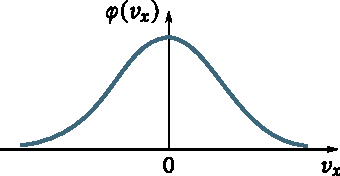
\includegraphics[scale=0.95]{figures/ch_11/fig_11_16.pdf}
			\caption[]{}
			\label{fig:11_16}
		\end{center}
	\end{minipage}
	\hspace{-0.05cm}
	\begin{minipage}[t]{0.5\linewidth}
		\begin{center}
			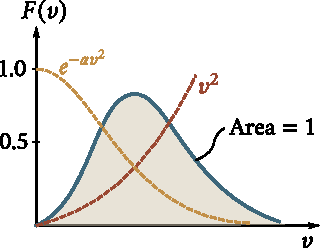
\includegraphics[scale=0.95]{figures/ch_11/fig_11_17.pdf}
			\caption[]{}
			\label{fig:11_17}
		\end{center}
	\end{minipage}
	\vspace{-0.7cm}
\end{figure}


Đồ thị của hàm~\eqref{eq:11_64} được cho trên hình \fig{11_17}. Vì khi tăng $v$, thừa số có dạng $e^{-\alpha v^2}$ giảm nhanh hơn sự tăng của thừa số $v^2$, nên hàm bắt đầu ở không (do $v^2$) sẽ đạt tới cực đại và sau đó tiến tới tiệm cận với không. Diện tích được bao quanh bởi đường cong là bằng một đơn vị so (so sánh với \eqn{11_7}).
Ta tìm vận tốc trung bình $\average{v}$ của các phân tử (ta đề cập đến vận tốc số học trung bình). Tương tự với  \eqn{11_9}, ta có:
\begin{equation*}
	\average{v} = \int_{0}^{\infty} vF(v)\,\deriv{v} = \left(\frac{m}{2\pi kT}\right)^{3/2} 4\pi \int_{0}^{\infty} \exp\left(-\frac{mv^2}{2kT}\right)\,v^2\,\deriv{v}.
\end{equation*}

\noindent
Chuyển sang biến số $\zeta=v^2$ và lấy tích phân từng phần sẽ dẫn đến kết quả sau:
\begin{equation}\label{eq:11_65}
	\average{v} = \left(\frac{8kT}{\pi m}\right)^{1/2}.
\end{equation}

Theo \eqn{11_11}
\begin{equation}\label{eq:11_66}
	\average{v^2} = \int_{0}^{\infty} v^2F(v)\,\deriv{v} = \left(\frac{m}{2\pi kT}\right)^{3/2} 4\pi \int_{0}^{\infty} \exp\left(-\frac{mv^2}{2kT}\right)\,v^4\,\deriv{v}.
\end{equation}

\noindent
Theo công thức \eqn{A_6}
\begin{equation*}
	\int_{0}^{\infty} \exp\left(-\frac{mv^2}{2kT}\right)\,v^4\,\deriv{v} = \frac{3}{8} \left(\frac{\pi}{(m/2kT)^5}\right)^{1/2} = \frac{3}{8\pi^2}\left(\frac{2\pi kT}{\pi}\right)^{5/2}.
\end{equation*}

\noindent

Thay thế giá trị này của tích phân vào \eqn{11_66} ta sẽ được đối với $\average{v^2}$ giá trị $3kT/m$ mà ta đã biết(xem \eqn{11_31}). Trong đó không có điều gì lạ, vì khi tìm giá trị của $\alpha$ trong \eqn{11_57} ta đã xuất phát từ hệ thức \eqn{11_32}, nghĩa là thực chất từ hệ thức \eqn{11_31}.

Căn bậc hai của $\average{v^2}$ được gọi là \textbf{vận tốc căn quân phương}:

\begin{equation}\label{eq:11_67}
	\ab{v}{qp} = \sqrt{\average{v^2}} = \left(\frac{3kT}{m}\right)^{1/2}.
\end{equation}
% vận tốc căn quân phương là v_{m sq}, và vận tốc xác suất lớn nhất bảng latex ghi là v_prob mình dịch là v_{xs} như bản scan 
Vận tốc ứng với cực đại của $F(v)$ sẽ có xác suất lớn nhất. Lấy đạo hàm của biểu thức \eqn{11_64} theo $v$, bỏ qua các thừa số không đổi và so sánh biểu thức thu được với không, ta đi tới phương trình
\begin{equation*}
	\exp\left(-\frac{mv^2}{2kT}\right)\left[2 - \frac{mv^2}{kT}\right] v = 0.
\end{equation*}

\noindent
Các giá trị $v=0$ và $v=\infty$ thõa mãn phương trình này tương ứng với các cực tiểu của $F(v)$. Giá trị của $v$, làm biểu thức đứng trong các dấu ngoặc triệt tiêu, là vận tốc có xác suất lớn nhất $\ab{v}{xs}$:
\begin{equation}\label{eq:11_68}
	\ab{v}{xs} = \left(\frac{2kT}{m}\right)^{1/2}.
\end{equation}

So sánh các biểu thức~\eqref{eq:11_65}, \eqref{eq:11_67}, và~\eqref{eq:11_67} cho ta
\begin{equation*}
	\ab{v}{xs}:\average{v}:\ab{v}{qp} = \sqrt{2}:\sqrt{8/\pi}:\sqrt{3} = 1 : 1.13 : 1.22.
\end{equation*}

\begin{figure}[!htb]
	\begin{minipage}[t]{0.5\linewidth}
		\begin{center}
			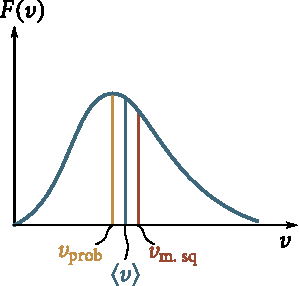
\includegraphics[scale=0.98]{figures/ch_11/fig_11_18.pdf}
			\caption[]{}
			\label{fig:11_18}
		\end{center}
	\end{minipage}
	\hspace{-0.05cm}
	\begin{minipage}[t]{0.5\linewidth}
		\begin{center}
			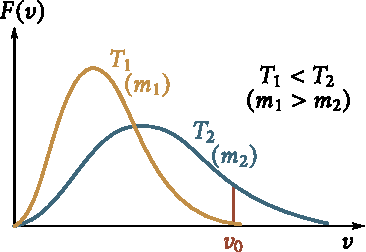
\includegraphics[scale=0.98]{figures/ch_11/fig_11_19.pdf}
			\caption[]{}
			\label{fig:11_19}
		\end{center}
	\end{minipage}
	\vspace{-0.4cm}
\end{figure}

\noindent
Hình~\ref{fig:11_18} minh họa cho hệ thức này.

Thay biểu thức \eqn{11_68} vào công thức~\eqref{eq:11_64} ta tìm được giá trị cực đại của hàm $F(v)$:
\vspace{-12pt} \\
\begin{equation}\label{eq:11_69}
	F(\ab{v}{xs}) = \frac{4}{e}\left(\frac{m}{2kT}\right)^{1/2} \propto \left(\frac{m}{T}\right)^{1/2}.
\end{equation}

\noindent
Từ công thức~\eqref{eq:11_68} và~\eqref{eq:11_69} suy ra rằng khi tăng nhiệt độ (hoặc khi giảm khối lượng của phân tử) cực đại của đường cong bị dịch chuyển sang phải và trở nên thấp hơn, thêm vào đó, như ta biết, diện tích được bao bởi đường cong vẫn không thay đổi. Trên hình~\ref{fig:11_19} người ta so sánh hai đường cong phân bố mà có thể giải thích chúng hoặc như đối với các nhiệt độ $T_1$ và $T_2$ (với $m$ như nhau) hoặc như đối với các khối lượng của các phân tử $m_1$ và $m_2$ khác nhau (với $T$ như nhau).

Số lượng tỷ đối với các phân tử có vận tốc vượt quá một giá trị $v_0$ nào đó được xác định bằng biểu thức 
\begin{equation*}
	\int_{v_0}^{\infty} F(v)\,\deriv{v}.
\end{equation*}

\noindent
Trên đồ thị phần diện tích giới hạn bởi đường cong nằm bên phải $v_0$ ứng với tích phân này. Từ hình vẽ \fig{11_19} rõ ràng là số lượng tỷ đối các phân tử có vận tốc vượt quá $v_0$ sẽ tăng mạnh với sự tăng nhiệt độ.

Trong bảng~\ref{table:11_3} ta đưa vào các số lượng tỷ đối các phân tử $\Delta N/N$ được tính nhờ hàm~\eqref{eq:11_64} đối với các khoảng khác nhau của vận tốc. Từ bảng suy ra rằng ở $70$\% tất cả các phân tử, vận tốc khác vận tốc có xác suất lớn nhất không quá $50$\%. Trung bình chỉ có $0.04$\% các phân tử có vận tốc vượt quá $\ab{v}{xs}$ hơn ba lần. Ngay cả các vận tốc vượt quá $5\ab{v}{xs}$ mà ta quan sát được thì trung bình cũng chỉ ở một trong 12 tỷ phân tử.

\begin{table}[!b]
	\renewcommand{\arraystretch}{1.2}
	\caption{ }
	\vspace{-0.6cm}
	\label{table:11_3}
	\begin{center}\resizebox{0.28\linewidth}{!}{
			\begin{tabular}{cc}
				\toprule[1pt]
				$v/\ab{v}{xs}$ & $\Delta N/N$, \%\\
				\midrule[0.5pt]\midrule[0.5pt]
				$0.0$-$0.5$ & $8.10$\\
				$0.5$-$1.5$ & $70.7$\\
				$1.5$-$2.0$ & $16.6$\\
				$2.0$-$3.0$ & $4.60$\\
				$>3.0$ 		& $0.04$\\
				$>5.0$ 		& \num{8e-9}\\
				\bottomrule[1pt]
			\end{tabular}
 	}\end{center}
\end{table}

Ta tiến hành đánh giá vận tốc trung bình của các phân tử Oxygen. Để tiến hành tính toán thuận lợi hơn, ta thay thế trong \eqn{11_65} tỷ số $k/m$ bằng tỷ số $R/M$ của nó. Khi đó biểu thức đối với vận tốc trung bình có dạng
\begin{equation}\label{eq:11_70}
	\average{v} = \left(\frac{8RT}{\pi M}\right)^{1/2}.
\end{equation}

\noindent

Khối lượng phân tử của oxygen là $32$. Do đó khối lượng của một mole là $M=\SI{32e-3}{\kilo\gram\per\mole}$. Nhiệt độ phòng là bằng khoảng \SI{300}{\kelvin}. Thay thế vào công thức \eqn{11_70} các trị số của các đại lượng tham gia vào công thức đó ta được 
\begin{equation*}
	\average{v} = \left(\frac{8 \times 8.31 \times 300}{3.14 \times 32\times10^{-3}}\right)^{1/2} \approx \SI{500}{\metre\per\second}.
\end{equation*}

\noindent

Vậy trung bình mỗi phân tử oxygen trong một giây đi qua một đoạn bằng \SI{0.5}{\kilo\metre}. Vì phân tử luôn luôn va chạm với các phân tử khác nên quãng đường này bao gồm một số lớn các đoạn thẳng ngắn tạo thành một đường gãy khúc.

Các phân tử hydrogen có khối lượng nhỏ hơn các phân tử oxygen $16$ lần, do đó vận tốc  của chúng ở cùng một nhiệt độ sẽ lớn hơn bốn lần và ở nhiệt độ phòng về trung bình là gần bằn \SI{2}{\kilo\metre\per\second}.

Nếu có một hỗn hợp các chất khí ở trạng thái cân bằng thì trong phạm vi các phân tử thuộc mỗi loại sẽ xảy ra sự phân bố~\eqref{eq:11_64} với giá trị $m$ của mình. Các phân tử nặng hơn về trung bình sẽ chuyển động với vận tốc nhỏ hơn vận tốc của các phân tử nhẹ hơn.


Xuất phát từ sự phân bố các phân tử theo các vận tốc
\begin{equation}\label{eq:11_71}
	\deriv{N_v} = N \left(\frac{m}{2\pi kT}\right)^{3/2} \exp\left(-\frac{mv^2}{2kT}\right) 4\pi v^2,\deriv{v}
\end{equation}

\noindent

có thể tìm được sự phân bố các phân tử theo các giá trị của động năng chuyển động tịnh tiến (ta ký hiệu nó bằng chữ $\varepsilon$). Muốn vậy cần chuyển từ biến số $v$ sang biến số $\varepsilon$ bằng $mv^2/2$. Thay thế $v=(2\varepsilon/m)^{1/2}$ và $\deriv{v}=(2m\varepsilon)^{-1/2}\,\deriv{\varepsilon}$ vào \eqn{11_71}, ta được 
\begin{equation}\label{eq:11_72}
	\deriv{N_{\varepsilon}} = N \frac{2}{\sqrt{\pi}} (kT)^{-3/2} \exp\left(-\frac{\varepsilon}{kT}\right) \varepsilon^{1/2}\,\deriv{\varepsilon}
\end{equation}

\noindent
Trong đó $\deriv{N_{\varepsilon}}$ là số phân tử mà động năng chuyển động tịnh tiến có các giá trị bao hàm trong phạm vi từ $\varepsilon$ đến $\deriv{\varepsilon}$.

Vậy sự phân bố các phân tử theo các giá trị $\varepsilon$ được đặc trưng bằng hàm

\begin{equation}\label{eq:11_73}
	f(\varepsilon) = A  \exp\left(-\frac{\varepsilon}{kT}\right) \varepsilon^{1/2}
\end{equation}

\noindent
trong đó $A$ là thừa số chuẩn hóa bằng $(2/\sqrt{\pi}) (kT)^{-3/2}$.

\section{Kiểm chứng bằng thực nghiệm định luật phân bố Maxwell}\label{sec:11_7}

Việc xác định bằng thực nghiệm đầu tiên các vận tốc của các phân tử được tiến hành bằng 0 đã được Stern thực hiện vào năm 1920. Dụng cụ được sử dụng vào mục đích này được tạo thành từ hai hình trụ đồng trục (\fig{11_20}). Một sợi dây platinum mạ bạc được căng theo trục của dụng cụ. Khi đốt nóng sợi dây bằng dòng điện thì các nguyên tử bạc được bốc ra từ bề mặt sợi dây. Các vận tốc của các nguyên tử được bốc ra tương ứng với nhiệt độ của sợi dây. Các nguyên tử chuyển động theo các hướng xuyên tâm sau khi rời khỏi sợi dây. Bên trong ống hình trụ có một khe dọc hẹp mà một chumg hẹp các nguyên tử đi qua đó ra ngoài (chùm phân tử). Để các nguyên tử bạc không bị lệch vì va chạm với các phân tử không khí thì toàn bộ dụng cụ phải được rút chân không. Sau khi đạt tới bề mặt ngoài của hình trụ, các nguyên tử bạc đọng lại trên đó tạo thành một lớp có dạng một dải thẳng đứng hẹp. 

\begin{figure}[!htb]
	\begin{center}
		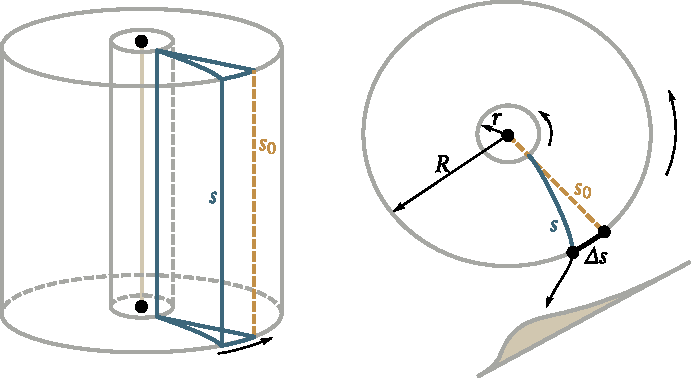
\includegraphics[scale=1.0]{figures/ch_11/fig_11_20.pdf}
		\caption[]{}
		\label{fig:11_20}
	\end{center}
	\vspace{-0.6cm}
\end{figure}

Nếu quay toàn bộ dụng cụ thì vết do chùm phân tử để lại bị dịch chuyển trên bề mặt ngoài hình trụ một khoảng $\Delta s$ nào đó(see \fig{11_20}). Điều này xảy ra vì trong thời gian mà các nguyên tử di chuyển qua lại giữa các khe hở giữa các hình trụ thì dụng cụ vừa quay đi một góc $\Delta\varphi$. Kêt quả là một phần khác của hình trụ ngoài bị dịch chuyển với vết ban đầu $s_0$ một lượng $\Delta s$ bằng $R\Delta\varphi$ ($R$ là bán kính của hình trụ ngoài) ngược với chùm. KHi xét chuyển động của các nguyên tử bạc trong hệ quy chiếu quay gắn với
các hình trụ, có thể giải thích sự dịch chuyển của vết bằng tác dụng của lực Coriolis bằng $2m(\vecprod{v}{\omega})$ lên các nguyên tử.

Có thể liên hệ khoảng cách $\Delta s$ giữa các dải bạc ban đầu và dải bạc bị dịch chuyển với vận tốc góc quay $\omega$ của các hình trụ bằng dạng hình học của dụng cụ, và vận tốc $v$ của các nguyên tử. Nếu kí hiệu thời gian bay bằng $\Delta t$, có thể viết là:

\begin{equation}\label{eq:11_74}
	\Delta s = \omega R\Delta t.
\end{equation}

\noindent
Vì bán kính hình trụ trong là nhỏ hơn so với bán kính hình trụ ngoài $R$, nên có thể đặt thời gian bay $\Delta t$ bằng
\begin{equation*}
	\Delta t = \frac{R}{v}.
\end{equation*}

\noindent
Thay biểu thức này vào \eqn{11_74} và giải phương trình thu được đối với $v$, ta được
\begin{equation*}
	v = \frac{\omega R^2}{\Delta s}.
\end{equation*}

Đo độ dịch chuyển của $\Delta s$ và vận tốc quay của dụng cụ có thể xác định được vận tốc $v$ của các nguyên tử. Thật vậy, tình huống sẽ bị phức tạp hóa là do sự phân bố theo các vận tốc, các nguyên tử sẽ có các vận tốc khác nhau. Kết quả là lớp dịch chuyển bị mờ \footnote {$\medskip$Bề rộng của lớp thu được khi dụng cụ đứng yên chỉ được xác định bằng hình dạng của dụng cụ, cụ thể là bằng bề rộng của khe mà chùm phân tử đi ra.}. Khi nghiên cứu mặt cắt nghiêng của vết (xem hình \fig{11_20}), Stern nhận thấy có thể hình thành một khái niệm gần đúng về cách các nguyên tử bạc được phân bố theo vận tốc.

Các kết quả của thí nghiệm của Stern đã khẳng định sự đúng đắn của việc đánh giá vận tốc trung bình của các nguyên tử mà ở đó vân tốc đó suy ra sự phân bố Maxwell. Tuy nhiên, thí nghiệm này chỉ có thể cung cấp thông tin rất gần đúng về bản chất của chính sự phân bố.

\begin{figure}[!htb]
	\begin{center}
		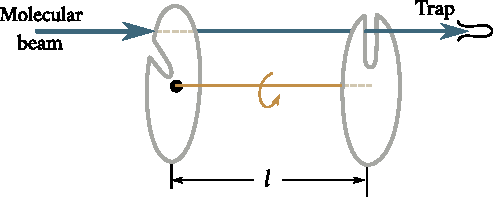
\includegraphics[scale=1.0]{figures/ch_11/fig_11_21.pdf}
		\caption[]{}
		\label{fig:11_21}
	\end{center}
	\vspace{-0.7cm}
\end{figure}

Một cách chính xác hơn, định luật phân bố đã được kiểm chứng chính xác hơn trong thí nghiệm do J. Lammert thực hiện (1929). Ông cho chùm phân tử qua hai đĩa quay có các khe xuyên tâm dịch chuyển so với nhau một góc $\varphi$ (\fig{11_21}). Trong số các phân tử bay qua khe ở đĩa thứ nhất sẽ chỉ có các phân tử bay tới đĩa thứ hai vào thời điểm khi rãnh ở đĩa thứ hai được đặt trước đường đi của chùm mới bay qua đĩa thứ hai. Các phân tử nhanh hơn sẽ đạt tới đĩa thứ hai quá sớm trong khi các phân tử chậm hơn thì quá trễ để đi qua. Do đó, cơ cấu này cho phép tách ra khỏi chùm, các phân tử có giá trị vận tốc xác định (do bề rộng hữu hạn của khe, dụng cụ sẽ tách các phân tử có vận tốc nằm trong phạm vi một khoảng $\Delta v$ nào đó). Vận tốc trung bình của các phân tử được dụng cụ tách ra có thể tìm được từ điều kiện là thời gian $t_1$ mà trong đó các phân tử bay qua khoảng cách $l$ giữa các đĩa ($t_1=l/v$) phải trùng với thời gian $t_2$ trong đó các đĩa quay một góc $\varphi$ (\ie, $t_1=\varphi/\omega$). So sánh cả hai thời gian ta được
\begin{equation*}
	v = \frac{\omega l}{\varphi}.
\end{equation*}

\noindent
Thay đổi vận tốc quay $\omega$ của dụng cụ (hoặc góc $\varphi$ giữa các đĩa), ta có thể tách khỏi chùm các phân tử có giá trị vận tốc khác nhau. Sau đó nếu thu được các phân tử này trong một khoảng thời gian xác định thì có thể xác định được số lượng tỉ đối của chúng trong chùm.

Các kết quả thí nghiệm của Lammert và các thí nghiệm khác được thực hiện với cùng một mục đích sẽ hoàn toàn phù hợp với định luật phân bố được Maxwell thành lập bằng lí thuyết.

Cần chú ý rằng, sự phân bố các phân tử theo các vận tốc trong chùm đi qua lỗ của bình sẽ hơi khác so với sự phân bố xảy ra trong một bình kín. Vì các phân tử nhanh hơn sẽ đi qua lỗ với một số lượng tương đối lớn hơn so với các phân tử chậm hơn, do đó chùm sẽ được lấp đầy bởi các phân tử nhanh hơn. Vì số lượng các phân tử bay qua lỗ trong một đơn vị thời gian tỉ lệ với $v$, nên sự phân bố trong chùm sẽ được đặc trưng không phải bằng hàm \eqref{eq:11_64}, mà là bằng hàm
\begin{equation*}
	F_1(v) = A_1 \exp\left(-\frac{mv^2}{2kT}\right) v^3
\end{equation*}

\noindent
Trong đó $A_1$ thừa số chuẩn hóa. Vận tốc có xác suất lớn nhất trong trường hợp này bằng $\ab{v}{xs}=\sqrt{3kT/m}$, và vận tốc trung bình bằng $\average{v'}=\sqrt{9\pi kT/8m}$.

\section{Phân bố Boltzmann}\label{sec:11_8}

Công thức khí áp thu được trong ~\eqref{eq:10_71} Sec.~\ref{sec:10_14}, \ie,
\begin{equation*}
	p = p_0 \exp\left(-\frac{Mgh}{RT}\right)
\end{equation*}

\noindent
cho sự phụ thuộc của áp suất vào độ cao trên mặt đất đối với sự đẳng nhiệt tưởng tượng của khí quyển. Thay thế trong số mũ của hàm mũ tỉ số $M/R$ bằng tỉ số $m/k$ ($m$ là khối lượng của phân tử, $k$ là hằng số Boltzmann). Ngoài ra, hãy đặt biểu thức $nkT$ thay cho $p$ và $n_0kT$ thay cho $p_0$ \eqn{10_21}. Sau đó lược cả hai vế của đẳng thức $kT$, ta được công thức
\begin{equation}\label{eq:11_75}
	n = n_0 \exp\left(-\frac{mgh}{kT}\right).
\end{equation}

\noindent
Trong đó $n$ là nồng độ phân tử (\ie, số phân tử trong một đơn vị phân tử) ở độ cao $h$, và $n_0$ là nồng độ phân tử ở độ cao $h_0=0$.

Từ công thức \eqn{11_75} suy ra rằng với sự hạ thấp nhiệt độ số hạt ở các độ cao khác 0 và trở về 0 khi $T=0$ (\fig{11_22}). Ở nhiệt độ 0 tuyệt đối, mọi phân tử đều có thể ở trên bề mặt Trái đất. Ngược lại, ở nhiệt độ cao, $n$ chỉ giảm đi một chút khi tăng độ cao để các phân tử phân bố theo độ cao gần như đồng đều.

\begin{figure}[!htb]
	\begin{center}
		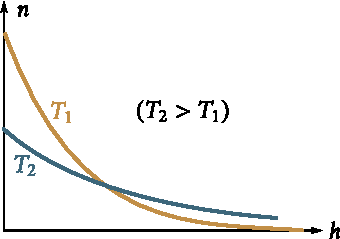
\includegraphics[scale=1.0]{figures/ch_11/fig_11_22.pdf}
		\caption[]{}
		\label{fig:11_22}
	\end{center}
	\vspace{-0.5cm}
\end{figure}

Điều này được giải thích một cách đơn giản bằng vật lý. Mỗi sự phân bố cụ thể của các phân tử theo độ cao đặt ra là kết quả do tác dụng của hai xu hướng: (1) sự hút các phân tử về Trái đất (được đặc trưng bằng lực $mg$) tiến tới sắp xếp các phần tử trên bề mặt Trái đất (2) chuyển động nhiệt (đặc trưng bằng đại lượng $kT$) tiến tới phân bố đều các phân tử theo tất cả các độ cao.  $m$ càng lớn và $T$ càng nhỏ thì xu hướng thứ nhất càng trội hơn, và các phân tử dày đặc ở bề mặt Trái đất. Tại giới hạn khi $T=0$, chuyển động nhieeth hoàn toàn dừng lại, và dưới ảnh hưởng của lực hút, các phân tử được phân bố trên bề mặt. Ở nhiệt độ cap, chuyển động nhiệt chiếm ưu thế, và mật độ của các phân tử giảm dần theo độ cao.

Ở các độ cao khác nhau, phân tử có dự trữ thế năng khác nhau:
\begin{equation}\label{eq:11_76}
	\ab{\varepsilon}{p} = mgh.
\end{equation}

\noindent
Do đó, sự phân bố của các phân tử theo độ cao cũng là sự phân bố của chúng theo các giá trị của thế năng. Nếu chú ý tới\eqn{11_76}, ta có thể viết \eqn{11_75} như sau:
\begin{equation}\label{eq:11_77}
	n = n_0 \exp\left(-\frac{\ab{\varepsilon}{p}}{kT}\right)
\end{equation}

\noindent
Trong đó $n$ là mật độ của các phân tử tại điểm trong không gian, mà tại đó thế năng của phân tử có giá trị $\ab{\varepsilon}{p}$ và $n_0$ là mật độ của các phân tử tại đó thế năng của phân tử bằng 0.

Từ \eqn{11_77} cho thấy rằng mật độ của các phân tử trên một đơn vị thể tích lớn hơn khi thế năng của chúng thấp hơn, và ngược lại, mật độ của chúng thấp hơn khi thế năng của chúng lớn hơn.

Theo \eqn{11_77}, tỉ số $n_1$ với $n_2$ tại những điểm mà thế năng của phân tử có giá trị $\ab{\varepsilon}{p,$1$}$ và $\ab{\varepsilon}{p,$2$}$ is
\begin{equation}\label{eq:11_78}
	\frac{n_1}{n_2} =  \exp\left[-\frac{\left(\ab{\varepsilon}{p,$1$} - \ab{\varepsilon}{p,$2$}\right)}{kT}\right].
\end{equation}

\noindent
L. Boltzmann đã chứng minh rằng~\eqref{eq:11_77} đối với một tập hợp những hạt đồng nhất bất kì ở trạng thái chuyển động nhiệt hỗn loạn, sự phân bố ở trên đúng không chỉ trong trường hợp trường thế của các lực hút của Trái đất mà còn cả trong một trường lực thế bất kì. Do đó, sự phân bố~\eqref{eq:11_77} được gọi là \textbf{sự phân bố Boltzmann}.

Trong khi định luật Maxwell cho biết sự phân bố của các hạt theo giá trị động năng của chúng, thì định luật Boltzmann cho biết sự phân bố của chúng theo giá trị thế năng. Cả hai phân bố được đặc trưng bởi sự hiện diện của một thừa số mũ mà số mũ là tỷ số giữa động năng hoặc một cách tương ứng của thế năng của một phân tử với đại lượng xác định năng lượng trung bình của chuyển động nhiệt của phân tử.

Theo công thức \eqn{11_77}, số lượng các phân tử nằm trong phạm vi thể tích $\deriv{V}=\deriv{x}\,\deriv{y}\,\deriv{z}$ đặt tại điểm có các tọa độ là $x, y, z$ is
\begin{equation}\label{eq:11_79}
	\deriv{N_{x,y,z}} = n_0 \exp\left[-\frac{\ab{\varepsilon}{p}(x,y,z)}{kT}\right]\,\deriv{x}\,\deriv{y}\,\deriv{z}.
\end{equation}

\noindent
Chúng ta lại thu được một biểu thức khác của luật phân phối Boltzmann.
Có thể hợp nhất các phân bố Maxwell và Boltzmann vào một định luật \textbf{Maxwell-Boltzmann} mà theo định luật đó số phần tử có các thành phần vận tốc nằm trong phạm vi từ $v_x, v_y, v_z$ tới $v_x+\deriv{v_x}, v_y+\deriv{v_y}, v_z+\deriv{v_z}$ và có tọa độ nằm trong giới hạn từ $x, y, z$ tới $x+\deriv{x}, y+\deriv{y}, z+\deriv{z}$ là bằng
\begin{equation}\label{eq:11_80}
	\deriv{N_{v_x,v_y,v_z,x,y,z}} = A \exp\left[-\frac{\left(\ab{\varepsilon}{p}+mv^2\right)}{kT}\right]\,\deriv{v_x}\,\deriv{v_y}\,\deriv{v_z}\,\deriv{x}\,\deriv{y}\,\deriv{z}
\end{equation}

\noindent
[xem Eqs.~\eqref{eq:11_40}, \eqref{eq:11_63}, và \eqref{eq:11_79}]. Ở đây, $A=n_0(m/2\pi kT)^{3/2}$, là thừa số chuẩn hóa. Nhớ rằng $\ab{\varepsilon}{p}=\ab{\varepsilon}{p}(x,y,z)$ và $v^2=v_x^2+v_y^2+v_z^2$.

Trong sự phân bố thế năng $\ab{\varepsilon}{p}$ và động năng $mv^2/2$, và do đó cả năng lượng toàn phần $E$, có thể nhận một loạt giá trị liên tục trong phân phối \eqref{eq:11_80}. Nếu tổng năng lượng của một hạt chỉ có thể nhận một chuỗi giá trị rời rạc $ E_1, E_2, \ ldots $, chẳng hạn như đối với nội năng của một nguyên tử, thì phân bố Boltzmann có dạng
\begin{equation}\label{eq:11_81}
	N_i = A \exp\left(-\frac{E_i}{kT}\right)
\end{equation}

\noindent
Trong đó $N_i$ là số hạt ở trạng thái với năng lượng $E_i$, $A$ là hệ số tỉ lệ phải thỏa mãn điều kiện $\sum_i N_i=A\sum_i\exp(-E_i/kT)=N$ ($N$ là tổng số hạt trong hệ được xét).

Thay giá trị của $A$ tìm được từ hệ thức này vào công thức \eqn{11_81}, ta thu được biểu thức cuối cùng của phân bố Boltzmann đối với trường hợp các giá trị năng lượng rời rạc:
\begin{equation}\label{eq:11_82}
	N_i = \frac{N \exp(-E_i/kT)}{\displaystyle\sum_i\exp(-E_i/kT)}.
\end{equation}

\section{Cách xác định số Avogadro của Perrin}\label{sec:11_9}

Sự phân bố \eqref{eq:11_75} đã được J.Perrin (1909) đặt làm cơ sở của các thí nghiệm về xác định hằng số Avogadro. Các hạt rắn rất nhỏ lơ lửng trong một chất lỏng sẽ ở trạng thái hỗn loạn không ngừng được gọi là chuyển động Brown (xem Sec.~\ref{sec:10_1}). Nguyên nhân của nó là với các hạt đủ nhỏ, mômen truyền cho một hạt do các phân tử va chạm với nó ở các phía khác nhau không cân bằng. Nếu một hạt có kích thước đáng kể, một số lượng lớn các phân tử va chạm với nó đồng thời, cho nên kết quả tổng của các va chạm của các phân tử sẽ khử lẫn nhau tức là các va chạm này bằng 0. Với các kích thước nhỏ, các hạt bắt đầu thể hiện các độ lệch khỏi các giá trị trung bình của vận tốc của các phân tử riêng biệt và của số phân tử va chạm. Nếu vận tốc hoặc số lượng phân tử va chạm với một hạt ở một bên khác với những phân tử va chạm với nó ở phía bên kia, thì động lượng kết quả truyền cho hạt sẽ khác 0, và hạt sẽ bắt đầu chuyển động trong hướng thích hợp. Tại thời điểm tiếp theo, động lượng tổng sẽ có một hướng khác. Do đó, hạt sẽ chuyển động hỗn loạn mọi lúc.

\begin{figure}[!htb]
	\begin{center}
		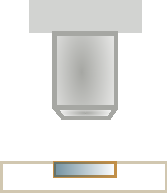
\includegraphics[scale=1.0]{figures/ch_11/fig_11_23.pdf}
		\caption[]{}
		\label{fig:11_23}
	\end{center}
	\vspace{-0.8cm}
\end{figure}

Chuyển động Brown chỉ ra rằng thực tế là các hạt đủ nhỏ tham gia vào chuyển động nhiệt do các phân tử thực hiện. Vì chúng tham gia vào chuyển động nhiệt, các hạt như vậy sẽ hoạt động giống như các phân tử khổng lồ, và chúng phải tuân theo các định luật của lý thuyết động học, đặc biệt là phân bố Boltzmann [xem \eqn{11_75}].

Khó khăn chính trong thí nghiệm của Perrin là việc chuẩn bị các hạt giống hệt nhau và xác định khối lượng của chúng. Bằng cách sử dụng nhiều lần phương pháp ly tâm, Perrin đã thành công trong việc điều chế một chất nhũ tương rất đồng nhất của các hạt gamboge gần như giống hệt nhau\footnote{$\medskip$Gamboge (cambogia) là một chất nhựa cao su đặc thu được từ các vết rạch trên vỏ của một số loài cây mọc ở Đông Dương và Shri Lanka.} với bán kính theo bậc của vài phần mười micromet. Nhũ tương được đặt trong khay thủy tinh phẳng \SI{0.1}{\milli\metre} sâu và được quan sát với sự hỗ trợ của kính hiển vi (\fig{11_23}).Kính hiển vi có trường độ sâu nhỏ đến mức chỉ có thể nhìn thấy các hạt trong lớp nằm ngang dày khoảng một micromet trong đó. Bằng cách di chuyển kính hiển vi theo phương thẳng đứng, người ta có thể nghiên cứu sự phân bố của các hạt Brown theo độ cao (chiều sâu).

 $h$ kí hiệu cho độ cao của lớp có thể nhìn thấy trong kính hiển vi phía trên đáy khay. Số lượng các hạt lọt vào tầm nhìn của kính hiển vi được xác định theo công thức
\begin{equation*}
	\Delta N = n(h) S \Delta h
\end{equation*}

\noindent
Trong đó $n(h)$ là số lượng các hạt Brown trong một đơn vị thể tích ở độ cao $h$, $S$ là diện tích và $\Delta h$ là trường độ sâu của kính hiển vi
Áp dụng công thức \eqn{11_75} cho các hạt Brown, có thể viết
\begin{equation*}
	n(h) = n_0 \exp\left(-\frac{p' h}{kT}\right)
\end{equation*}

\noindent
trong đó $n_0$ là số hạt trong một đơn vị thể tích $h=0$, và $p'$ là trọng lượng của hạt Brown trong chất nhũ tương, \ie, nghĩa là trọng lượng được lấy khi kể đến sự hiệu chỉnh về định luật Archimedes.

Viết biểu thức số hạt $\Delta N$ đối với hai độ cao khác nhau $h_1$ và $h_2$, ta được
\begin{align*}
	\Delta N_1 &= n_0 \exp\left(-\frac{p' h_1}{kT}\right) S \Delta h,\\
	\Delta N_2 &= n_0 \exp\left(-\frac{p' h_2}{kT}\right) S \Delta h.
\end{align*}

\noindent
Cuối cùng, lấy logarit của tỷ lệ $\Delta N_1/\Delta N_2$, ta đi đến biểu thức sau:
\begin{equation}\label{eq:11_83}
	\ln\left(\frac{\Delta N_1}{\Delta N_2}\right) = \frac{p' (h_2 - h_1)}{kT}.
\end{equation}

Dựa vào công thức này $p'$, $T$, $(h_2-h_1)$, $\Delta N_1$, và $\Delta N_2$, \eqn{11_83} có thể xác định hằng số Boltzmann theo $k$. Hơn nữa, chia hằng số khí $R$ cho $k$, có thể tìm được hằng số Avogadro $\ab{N}{A}$.

Giá trị $\ab{N}{A}$ do Perrin thu được trên các nhũ tương khác nhau nằm trong phạm vi từ \SIrange{6.5e23}{7.2e23}{\per\mole}. Giá trị của nó được xác định bằng các phương pháp khác chính xác hơn là\SI{6.02e23}{\per\mole}. Do đó giá trị thu được của Perrin khá phù hợp với các giá trị thu được bằng các phương pháp khác. Điều này chứng tỏ khả năng áp dụng phân bố Boltzmann cho các hạt Brown.

\section{Các trạng thái vĩ mô và vi mô. Trọng số thống kê}\label{sec:11_10}

Trạng thái của một vật vĩ mô (nghĩa là vật được tạo thành bởi một lượng khổng lồ các phân tử) có thể được tạo thành dựa vào khối lượng, áp suất, nhiệt độ, năng lượng bên trong và các vĩ mô khác (nghĩa là các đại lượng đặc trưng cho tất cả các vật xét về toàn bộ). Trạng thái đặc trưng bằng cách như thể được gọi là  \textbf{trạng thái vĩ mô}.

Trạng thái của một vật vĩ mô được đặc trưng chi tiết đến mức trạng thái của tất cả các phân tử tạo thành cơ thể được thiết lập được định nghĩa là \textbf{trạng thái vi mô}.

Một trạng thái vĩ mô có thể đạt được theo nhiều cách khác nhau mà mỗi cách ứng với một trạng thái vĩ mô nào đó của vật. Số trạng thái vi mô khác nhau ứng với một trạng thái vĩ mô đã cho được gọi là \textbf{trọng số thống kê} hoặc \textbf{xác suất nhiệt động học} của trạng thái vĩ mô. Vậy, trọng số thống kê là số cách vi mô mà trạng thái vĩ mô đã cho có thể thực hiện.

Để làm rõ khái niệm trọng lượng thống kê, chúng ta hãy xem xét các cách mà các phân tử của một chất khí có thể được phân bố giữa hai nửa của bình chứa chất khí đó. Giả sử tổng số phân tử bằng $N$. Để đặc trưng cho trạng thái của chất khí, ta lấy số phân tử ở nửa bình bên trái mà được kí hiệu bằng chữ $n$ (một cách tương ứng, số phân tử ở nửa bình bên phải sẽ kí hiệu là $N-n$).Ta sẽ mô tả trạng thái của một phân tử riêng lẻ bằng cách cho biết nó đang ở trong nửa bình nào. Việc mô tả như vậy về trạng thái của một chất khí và trạng thái của các phân tử riêng lẻ của nó đương nhiên là không hoàn chỉnh. Nhưng nó đủ để giải thích các tính chất đặc trưng về hành vi thống kê của bất kỳ hệ thống vĩ mô nào bằng cách sử dụng ví dụ này.

\begin{figure}[!htb]
	\begin{center}
		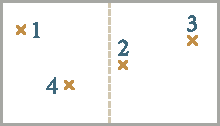
\includegraphics[scale=1.0]{figures/ch_11/fig_11_24.pdf}
		\caption[]{}
		\label{fig:11_24}
	\end{center}
	\vspace{-0.8cm}
\end{figure}

Chúng ta hãy bắt đầu với trường hợp tổng số phân tử bằng bốn (\fig{11_24}). Mỗi phân tử có thể nằm ở nửa bên trái hoặc nửa bên phải của bình với xác suất bằng nhau. Do đó, xác suất của, giả sử, phân tử $1$ nằm ở nửa bình bên trái là $1/2$. Sự lưu lại ở nửa bình bên trái của phân tử $1$ và sự lưu lại ở cùng nửa bình đó của phân tử $2$ là các biến cố độc lập thống kê với nhau. Do đó, xác suất để tìm được đồng thời các phân tử $1$ và $2$ ở phần bên trái của bình là bằng tích các xác suất, nghĩa là, $(1/2)^2$. Tiếp tục các lập luận này ta thu được xác suất tìm được đồng thời tất cả bốn phân tử ở nửa bình bên trái là bằng $(1/2)^4$.

Suy luận tương tự cho thấy rằng xác suất của bất kỳ sự sắp xếp nào của các phân tử trong bình (giả sử, một trong đó các phân tử $1$ và $4$nằm ở nửa bên trái và các phân tử $2$ và $3$ ở bên phải) cũng bằng $(1/2)^4$.Mỗi cách sắp xếp là một vi hạt của khí. Từ những gì đã nói ở trên, xác suất của tất cả các vi hạt là như nhau và bằng $(1/2)^4$.

Bảng \ref{table:11_4} cho thấy tất cả các cách có thể để phân phối các phân tử giữa các nửa của bình (tất cả các vi hạt của khí). Chẳng hạn, trạng thái được đặc trưng bằng điều là ở phần nửa bên trái của bình có một phân tử (phân tử nào cũng được) và nửa bên phải có ba phân tử là một trạng thái vĩ mô. Kiểm tra bảng cho thấy rằng bốn trạng thái vi mô tương ứng với một trạng thái vĩ mô như vậy. Do đó, trọng số thống kê của trạng thái vĩ mô đã cho là bằng $4$, và xác suất (thông thường, và không phải nhiệt động lực học) là $4/16$. Một trạng thái vĩ mô mà trong đó cả hai nửa của bình chứa cùng một số lượng phân tử được thực hiện với sự hỗ trợ của sáu trạng thái vi mô. Trọng lượng thống kê của nó là phù hợp $6$, và xác suất của nó (thông thường) là $6/16$.

\begin{table}[!b]
	\renewcommand{\arraystretch}{1.2}
	\caption{ }
	\vspace{-0.6cm}
	\label{table:11_4}
	\begin{center}\resizebox{0.80\linewidth}{!}{
			\begin{tabular}{p{1.8cm}p{1.8cm}p{1.8cm}p{1.8cm}c}
				\toprule[1pt]
				\multicolumn{2}{c}{\textbf{Trạng Thái}} & \multicolumn{2}{c}{\textbf{Các cách thực hiện trạng thái}} & \multirow{2}{2.45cm}{\textbf{Số cách thực hiện trạng thái đã cho($\Omega$)}}\\ \\
				\cline{1-2}\cline{3-4}
				\textbf{Số phân tử ở bên trái} & \textbf{Số phân tử ở bên phải} &
				\textbf{Số phân tử ở bên trái} & \textbf{Số phân tử ở bên phải} \\
				\midrule[0.5pt]\midrule[0.5pt]
				$0$&$4$&---&$1,2,3,4$&$1$\\
				\midrule[0.5pt]
				\multirow{4}{*}{$1$}&\multirow{4}{*}{$3$}&$1$&$2,3,4$&\multirow{4}{*}{$4$}\\
				& & $2$ & $1,3,4$ &\\
				& & $3$ & $1,2,4$ &\\
				& & $4$ & $1,2,3$ &\\
				\midrule[0.5pt]
				\multirow{6}{*}{$2$}&\multirow{6}{*}{$2$}&$1,2$&$3,4$&\multirow{6}{*}{$6$}\\
				& & $1,3$ & $2,4$ &\\
				& & $1,4$ & $2,3$ &\\
				& & $2,3$ & $1,4$ &\\
				& & $2,4$ & $1,3$ &\\
				& & $3,4$ & $1,2$ &\\
				\midrule[0.5pt]
				\multirow{4}{*}{$3$}&\multirow{4}{*}{$1$}&$1,2,3$&$4$&\multirow{4}{*}{$4$}\\
				& & $1,2,4$ & $3$ & \\
				& & $1,3,4$ & $2$ & \\
				& & $2,3,4$ & $1$ & \\
				\midrule[0.5pt]
				$4$ & $0$ & $1,2,3,4$ & --- & $1$\\
				\midrule[0.5pt]
				\multicolumn{4}{c}{Tất cả các cách} & $2^4=16$\\
				\bottomrule[1pt]
			\end{tabular}
	}\end{center}
\end{table}

Ví dụ trên cho thấy rằng tất cả các trạng thái vi mô của một hệ thống nhất định đều có thể xảy ra như nhau. Do đó, trọng số thống kê tỷ lệ với xác suất (quy ước) của trạng thái vĩ mô. Tuyên bố rằng tất cả các vi hạt đều có khả năng xảy ra như nhau là nền tảng của vật lý thống kê và được gọi là \textbf{giả thiết ergodic}.

Theo như bảng \ref{table:11_4}, khi chúng ta xử lý bốn phân tử, xác suất tất cả các phân tử tập hợp ở một trong hai nửa (trái hoặc phải) của bình là khá lớn (1/8). Tuy nhiên, các vấn đề thay đổi đáng kể với sự gia tăng số lượng phân tử.

Ta tìm số cách. (số trạng thái vi mô) mà nhờ chúng có thể thực hiện được một trạng thái vĩ mô được đặc trưng bằng điều là ở nửa bình bên trái là $n$ phân tử trong tổng số $N$ của chúng, còn ở nửa bên phải là $N-n$ phân tử. Muốn vậy ta đánh số các phân tử bằng cách viết cho chúng các số thứ tự từ $1$ đến $N$. Sau đó,  ta sẽ lấy từng phân tử một và đặt nó vào nửa bên trái của bình. Có thể chọn phân tử thứ nhất bằng $N$ cách, phân tử thứ hai bằng $N-1$ cách, phân tử thứ ba bằng $N-2$ cách, cuối cùng, phân tử thứ $n$ có thể chọn bằng $N-n+1$ cách. Ta xếp $N-n$ phân tử còn lại vào nửa bình bên phải

Từ điều đã nêu ở trên suy ra rằng số $z$ cách mà nhờ chúng có thể chọn một cách ngẫu nhiên $n$ phân tử trong tổng số $N$ phân tử cho nửa bình bên trái sẽ bằng:
\begin{equation*}
	z = N(N-1)(N-2)\ldots (N-n+1).
\end{equation*}

\noindent
Nhân và chia số đó với $(N-n)!$, ta được
\begin{equation}\label{eq:11_84}
	z = \frac{N!}{(N-n)!}.
\end{equation}

Tuy nhiên không phải tất cả $z$ cách chọn đều dẫn tới các trạng thái vi mô khác nhau, tuy nhiên, các trạng thái vi mô tách biệt chỉ khác nhau bởi tập hợp số thứ tự các phân tử được chọn cho mỗi nửa bình mà không phải bởi sự kế tiếp nhau, theo đó ta đã chọn các phân tử đó. Chẳng hạn, với $N=3$ và $n=2$, ta có các cách chọn
\begin{align*}
	&\!\! 1\text{-}2\quad 2\text{-}1\quad 3\text{-}1\\
	&\!\! 1\text{-}3\quad 2\text{-}3\quad 3\text{-}2.
\end{align*}

\noindent
Trong các cách chọn $1$-$2$ và $2$-$1$ ứng với cùng một trạng thái vi mô (các phân tử $1$ và $2$ vào nửa bên trái và phân tử $3$ vào nửa bên phải). Tương tự với các cách chọn $1$-$3$ và $3$-$1$, cũng như $2$-$3$ và $3$-$2$. Do vậy, các cách chọn chỉ khác nhau bởi các hoán vị $n$ số thứ tự các phân tử được chọn cho nửa bình bên trái ($n!$ cách chọn như vậy) tương ứng với cùng một trạng thái vi mô. Do đó, để có được trạng thái vi mô mà nhờ chúng trạng thái vĩ mô ($n$, $N-n$), có thể được thực hiện cần phải chia số $z$ có trong \eqn{11_84} cho $n!$. Kết quả là đối với trọng số thống kê ta có biểu thức
\begin{equation}\label{eq:11_85}
	\Omega(n, N-n) = \frac{N!}{n!(N-n)!}.
\end{equation}

\noindent
Dễ dàng thấy rằng $\Omega(2, 4-2)=6$, and $\Omega(1, 4-1)=4$ (see Table~\ref{table:11_4}).

Bảng \ref{table:11_5} đưa vào các giá trị $\Omega$ được tính theo công thức \eqn{11_85} với trường hợp $N=24$.

\begin{table}[!b]
	\renewcommand{\arraystretch}{1.2}
	\caption{ }
	\vspace{-0.6cm}
	\label{table:11_5}
	\begin{center}\resizebox{0.98\linewidth}{!}{
			\begin{tabular}{ccrrccrr}
				\toprule[1pt]
				\multicolumn{2}{c}{\textbf{Số phân tử}} & \multirow{2}{1.3cm}{\hfill{ }$\Omega$} & \multirow{2}{1.8cm}{\hfill{ }Xác suất} & \multicolumn{2}{c}{\textbf{Số phân tử}} & \multirow{2}{1.3cm}{\hfill{ }$\Omega$} & \multirow{2}{1.8cm}{\hfill{ }Xác suất}\\
				\cline{1-2}\cline{5-6}
				\textbf{Trái} & \textbf{Phải} & & &
				\textbf{Trái} & \textbf{Phải} & & \\
				\midrule[0.5pt]\midrule[0.5pt]
				$0$ & $24$ & $1$ & \num{6.0e-7} & $9$ & $15$ & $1307504$ & \num{7.8e-2}\\
				$1$ & $23$ & $24$ & \num{1.4e-6} & $10$ & $14$ & $1961256$ & \num{0.117}\\
				$2$ & $22$ & $276$ & \num{1.6e-5} & $11$ & $13$ & $2496144$ & \num{0.149}\\
				$3$ & $21$ & $2024$ & \num{1.2e-4} & $12$ & $12$ & $2704156$ & \num{0.161}\\
				$4$ & $20$ & $10626$ & \num{6.3e-4} & $13$ & $11$ & $2496144$ & \num{0.149}\\
				$5$ & $19$ & $42504$ & \num{2.5e-3} & \ldots & \ldots & \ldots & \ldots\\
				$6$ & $18$ & $134596$ & \num{8.0e-3} & $23$ & $1$ & $24$ & \num{1.4e-6}\\
				$7$ & $17$ & $346104$ & \num{2.0e-2} & $24$ & $0$ & $1$ & \num{6.0e-7}\\
				$8$ & $16$ & $735471$ & \num{4.4e-2} &  &  & & \\
				\midrule[0.5pt]
				\multicolumn{8}{c}{Tổng $2^{24} = 16777216$ cách}\\
				\bottomrule[1pt]
			\end{tabular}
	}\end{center}
\end{table}

Tổng số cách phân bố $24$ phân tử giữa hai nửa bình là bằng $2^{24}=16777216$, và tất cả các phân tử tập trung vào một nửa bình chỉ duy nhất trong hai trường hợp. Xác suất của một biến cố như vậy bằng khoảng \num{e-7}. Trong 4 centimet khối không khí có chứa khoảng \num{e20} phân tử. Xác suất để tất cả các phân tử này tập trung vào một nửa bình là bằng 2 chia cho 2 lũy thừa  \num{e20}, tổng cộng là gần bằng $10^{-3\times10^{19}}$. Xác suất này nhỏ đến mức thực tế có thể coi nó bằng $0$ 

\begin{figure}[!htb]
	\begin{center}
		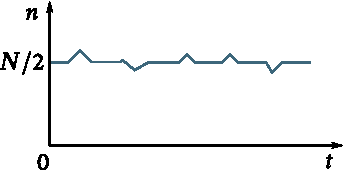
\includegraphics[scale=1.0]{figures/ch_11/fig_11_25.pdf}
		\caption[]{}
		\label{fig:11_25}
	\end{center}
	\vspace{-0.8cm}
\end{figure}

Trên hình \ref{fig:11_25} biểu diễn đồ thị chứng tỏ phân tử     $n$ ở một nửa bình bị biến đổi như thế nào với thời gian. Con số này dao động xung quanh giá trị trung bình bằng $N/2$. Các độ lệch ngẫu nhiên của các giá trị của một đại lượng vật lí $x$ nào đó khỏi giá trị trung bình $\average{x}$ của nó được gọi là các độ thăng giáng của đại lượng này. Kí hiệu là $\Delta x$, ta thu được
\begin{equation}\label{eq:11_86}
	\Delta x = x - \average{x}.
\end{equation}

\noindent
Số trung bình cộng của đại lượng \eqref{eq:11_86} = $0$. Thực vậy,
\begin{equation*}
	\average{\Delta x} = \average{(x - \average{x})} = \average{x} - \average{x} = 0.
\end{equation*}

\noindent
Do đó để đặc trưng cho độ thăng giáng người ta lấy \textbf{bình phương trung bình} bằng
\begin{equation}\label{eq:11_87}
	\bracket{\average{(\Delta x)^2}}^{1/2}.
\end{equation}

Sự biến động tương đối của số lượng $x$ mang tính biểu thị nhiều hơn. Nó được xác định bởi tỷ lệ
\begin{equation}\label{eq:11_88}
	\frac{\bracket{\average{(\Delta x)^2}}^{1/2}}{\average{x}}.
\end{equation}

Trong vật lý thống kê, người ta chứng minh rằng sự dao động tương đối của một đại lượng cộng tính (nghĩa là, một đại lượng mà giá trị của nó đối với một vật là bằng tổng các giá trị đối với các phần riêng biệt của nó) là tỉ lệ nghịch với căn bậc hai của số $N$ phân tử tạo thành vật:
\begin{equation}\label{công thức:11_89}
	\frac{\bracket{\average{(\Delta x)^2}}^{1/2}}{\average{x}} \propto \frac{1}{N^{1/2}}.
\end{equation}

Hãy tính toán sự dao động tương đối của số lượng phân tử trong nửa bên trái của bình bằng cách sử dụng dữ liệu của bảng \ref{table:11_4}. Thực hiện cách tính bằng công thức \eqn{11_5}. Giá trị của các biến động và xác suất của chúng $P$ được đưa ra dưới đây.
\begin{align*}
	n-N/2 & \ldots \quad -2 \quad -1 \quad 0 \quad +1 \quad +2\\
	P & \ldots \quad 1/16 \quad 4/16 \quad 6/16 \quad 4/16 \quad 1/16
\end{align*}

Theo các dữ kiện này
\begin{align*}
	\average{(n-N/2)^2} = (-2)^2 \times 1/16 + (-1)^2 \times 4/16 &+ (0)^2 \times 6/16 \\
	(+1)^2 \times &4/16 + (+2)^2 \times 1/16 = 1.
\end{align*}

\noindent
Do đó, độ thăng giáng bình phương bằng $\sqrt{1}=1$, và độ thăng giáng tỉ đối bằng $1/2$ (giá trị trung bình của $n$ là $2$). Các phép tính tương tự được thực hiện dựa vào dữ kiện của bảng \ref{table:11_5} cho giá trị $2.45$ đối với độ thăng giáng bình phương, và $0.204$ đối với độ thăng giáng tỉ đối. Dễ thấy rằng
\begin{equation}\label{eq:11_90}
	0.5 : 0.204 = \sqrt{24 : 4}.
\end{equation}

\noindent
Hệ thức này phù hợp với công thức \eqn{11_89}.

Từ bảng \ref{table:11_5} suy ra rằng độ lệch số trung bình của các phân tử (bằng $12$) không lớn hơn $2$ phân tử được thực hiện với xác suất $0.7$, và độ lệch không lớn hơn $3$ phân tử với xác xuất $0.85$. Nếu số lượng phân tử có thể được chia nhỏ, ta có thể nói rằng phần lớn thời gian chất khí ở trạng thái mà trong đó độ lệch của số lượng phân tử so với giá trị trung bình không vượt quá dao động tương đối, nghĩa là, $2.45$.

Thành lập tỉ lệ, tương tự như \eqref{eq:11_90} đối với $N=4$ và $N=\num{e20}$, thu được độ tăng giáng tỉ đối ($\ab{f}{r}$) của số phân tử ở nửa bình bên trái trong trường hợp $N=\num{e20}$. Tỉ lệ này có dạng
\begin{equation*}
	0.5 : \ab{f}{r}=\sqrt{\num{e20} : 4}
\end{equation*}

\noindent
Từ đó $\ab{f}{r}=\num{e-10}$. Kết quả thu được cho thấy rằng giá trị của số phân tử ở một trong hai nửa của bình bị thay đổi, về cơ bản không vượt quá một đơn vị của chữ số có nghĩa thứ mười

Ta đã xem xét sự dao động của số lượng phân tử của một trong hai nửa của chiếc bình. Các đặc điểm vĩ mô khác như áp suất và mật độ của khí tại các điểm khác nhau trong không gian cũng dao động, tức là, lệch khỏi giá trị trung bình của chúng.

Trạng thái vĩ mô của một hệ thống là trạng thái cân bằng khi nó không có xu hướng thay đổi theo thời gian. Rõ ràng rằng sự vắng mặt của một xu hướng như vậy sẽ được thể hiện lớn nhất trong những điều có thể xảy ra nhất trong tất cả các chỉ số vĩ mô có thể tưởng tượng được đối với hệ thống đã cho. Xác suất của một trạng thái tỷ lệ với trọng số thống kê của nó. Do đó, trạng thái cân bằng có thể được xác định là trạng thái có trọng số thống kê là cực đại.

Hệ ở trạng thái cân bằng bị lệch khỏi trạng thái cân bằng một cách tự phát theo thời gian. Tuy nhiên, những sai lệch này là không đáng kể và không kéo dài. Phần lớn thời gian của nó ở trạng thái cân bằng được đặc trưng bởi trọng số thống kê cực đại.

Vật lý thống kê tiết lộ bản chất của các quá trình không thể đảo ngược. Giả sử rằng đầu tiên một chất khí nằm trong nửa bên trái của bình được ngăn cách bởi vách ngăn với nửa trống bên phải. Nếu chúng ta loại bỏ vách ngăn, khí sẽ tự phát lan ra toàn bộ bình. Quá trình này sẽ không thể đảo ngược bởi vì xác suất của thực tế là do chuyển động nhiệt tất cả các phân tử sẽ tập trung lại ở một trong các nửa của bình, như chúng ta đã thấy, hầu như là không. Do đó, khí không thể tự tập trung ở nửa bên trái của bình mà không có bất kỳ tác động bên ngoài nào lên nó.

Do đó, quá trình lan truyền của khí trên toàn bộ bình là không thuận nghịch vì quá trình ngược lại với nó có xác suất nhỏ. Kết luận này cũng có thể được mở rộng cho các quá trình khác. Mỗi quá trình không thuận nghịch - đó là quá trình mà quá trình ngược với nó có xác xuất cực kì nhỏ

\section{Entropy}\label{sec:11_11}

Ta đã thiết lập ở phần trước rằng xác suất của một trạng thái vĩ mô (ở phần sau chúng ta sẽ gọi nó đơn giản là xác suất trạng thái) tỷ lệ với trọng số thống kê $\Omega$ của nó, nghĩa là số các cách vi mô của chúng có thể thực hiện trạng thái vĩ mô đã cho. Do đó, có thể lấy chính số này, tức là $\Omega$, để đặc trưng cho xác suất trạng thái. Tuy nhiên, một đặc tính như vậy sẽ không có tính chất cộng hưởng. Để thấy rõ điều này, ta hãy chia một hệ đã cho thành hai hệ con hầu như không tương tác với nhau. Hãy để các hệ con này ở trạng thái có trọng số thống kê $\Omega_1$ và $\Omega_2$. Số cách mà chúng ta có thể đạt được trạng thái tương ứng của hệ bằng tích của số cách mà chúng ta có thể đạt được trạng thái của từng hệ con riêng biệt:
\begin{equation}\label{công thức:11_91}
	\Omega = \Omega_1\Omega_2.
\end{equation}

\noindent
Từ đó suy ra rằng $\Omega$ thực tế không phải là một đại lượng cộng tính

Lấy logarit hệ thức \eqn{11_91}, ta được
\begin{equation}\label{công thức:11_92}
	\ln{\Omega} = \ln{\Omega_1} + \ln{\Omega_2}.
\end{equation}

\noindent
Từ \eqn{11_92} rõ ràng $\ln{\Omega}$ là một đại lượng cộng tính. Đề cập đến các đại lượng cộng tính thì đơn giản và thuận lợi hơn nhiều. Do đó để đặc trưng cho xác suất trạng thái, người ta sử dụng đại lượng $S$ tỉ lệ với logarit của trọng số thống kê. Theo lí do mà ta sẽ giải thích dưới đây, người ta chọn hệ số tỉ lệ bằng hằng số Boltzmann $k$. Đại lượng
\begin{equation}\label{công thức:11_93}
	S = k \ln{\Omega}
\end{equation}

\noindent
được xác định theo cách này được gọi là \textbf {entropy} của một hệ.

Các thuộc tính của entropy được chỉ ra dưới đây tuân theo những gì đã nói trong phần trước:
\begin{enumerate}[1.]
	\item Entropy của một hệ cô lập phát triển khi một quá trình không thuận nghịch xảy ra trong nó. Thật vậy, một hệ thống cô lập (tức là một hệ thống còn lại của chính nó) chuyển từ trạng thái có khả năng xảy ra thấp hơn sang trạng thái có khả năng xảy ra cao hơn, và điều này có sự tăng trưởng của số lượng \eqref{eq:11_93}.
	\item Entropy của hệ ở trạng thái cân bằng là cực đại
\end{enumerate}

Ta sẽ nhấn mạnh một lần nữa tính chất chặt chẽ một cách không hoàn toàn tuyệt đối của các điều khẳng định đã trình bày ở trên. Ví dụ, entropi của một hệ thống ở trạng thái cân bằng trải qua những dao động giáng âm ngắn hạn không đáng kể. Tuy nhiên, giá trị thứ hai nhỏ đến mức entropy hầu như có thể được coi là không đổi và bằng giá trị cực đại.

Khẳng định rằng entropy của một hệ cô lập chỉ có thể lớn lên (hoặc không đổi khi đạt đến giá trị lớn nhất) được gọi là \textbf {định luật tăng entropy} hoặc \textbf {định luật thứ hai của nhiệt động lực học}. Nói cách khác, chúng ta có thể nói rằng entropy của một hệ cô lập không thể giảm.

Do đó, khi quá trình thuận nghịch xảy ra trong một hệ thống cô lập, entropy tăng lên, tức là, mối quan hệ sau đây được quan sát thấy:
\begin{equation}\label{công thức:11_94}
	\deriv{S} > 0.
\end{equation}

Để xem entropy của một hệ không cô lập hoạt động như thế nào, chúng ta hãy thiết lập mối quan hệ giữa số gia của entropy $\deriv{S}$ và nhiệt lượng $\derivp{Q}$ cung cấp cho hệ. Entropi phải được xác định bởi các tham số về trạng thái của một vật (hoặc một hệ thống các vật). Một chất khí lý tưởng có những tính chất đơn giản nhất. Trạng thái cân bằng của nó hoàn toàn được xác định bằng cách thiết lập hai thông số, ví dụ, thể tích $V$ và nhiệt độ $T$. Chúng ta hãy thử tìm dạng của hàm $S = S(V,T)$ cho một khí lý tưởng đơn nguyên tử \footnote {$\medskip$Đạo hàm sau đây được đề xuất bởi N. B. Narozhny.}.

Ta sẽ xem xét một khí lý tưởng về mặt cấu tạo ở trạng thái cân bằng trong một bình thể tích $V$. Xem rằng các trường lực ngoài không có mặt. Số phân tử trong chất khí là $N$ và nhiệt độ của nó là $T$. Trạng thái vĩ mô của chất khí được đặc trưng bởi các giá trị của các tham số $V$ và $T$, và trạng thái vi mô của nó được xác định bằng cách thiết lập tọa độ và vận tốc của tất cả các phân tử $N$. Sự phân bố của các phân tử theo tọa độ và sự phân bố của chúng theo vận tốc là độc lập. Do đó, trọng số thống kê $\Omega$ của một trạng thái vĩ mô có thể được biểu diễn dưới dạng tích của thừa số $\ab{\Omega}{sp}$ xác định số lượng các cách sắp xếp (hoán vị) khác nhau của các phân tử trong không gian, và hệ số $\ab{\Omega}{v}$ xác định số lượng phân bố khác nhau của các phân tử theo vận tốc:
\vspace{-12pt}

\begin{equation}\label{công thức:11_95}
	\Omega = \ab{\Omega}{sp} \ab{\Omega}{v}.
\end{equation}

\noindent
Thực vậy, mỗi cách sắp xếp $\ab{\Omega}{sp}$ trong không gian có thể thực hiện đồng thời với một phân bố bất kì trong $\ab{\Omega}{v}$ nào theo vận tốc. Từ đó suy ra công thức \eqn {11_95}.

Do đó, trong trường hợp đang xét, biểu thức cho entropi có dạng
\vspace{-12pt} \\
\begin{equation}\label{công thức:11_96}
	S = k \ln{\Omega} = k \ln{\ab{\Omega}{sp}} + k \ln{\ab{\Omega}{v}}.
\end{equation}

\noindent
Từ phương trình này có thể thấy rằng việc tìm ra entropi của khí lý tưởng bao gồm việc tìm các số $\ab{\Omega}{sp}$ và $\ab{\Omega}{v}$. Sau khi xác định những con số này phụ thuộc như thế nào vào các tham số $V$ và $T$ của một chất khí, ta sẽ tìm entropy của nó như một hàm của các tham số này.

Để xác định số $ \ab{\Omega}{sp}$, ta hãy chia thể tích $V$ chứa chất khí thành các ô hình khối giống hệt nhau. Ta sẽ chọn thể tích của ô $\Delta V$ để số ô
\begin{equation}\label{công thức:11_97}
	r = \frac{V}{\Delta V}
\end{equation}

\noindent
nhỏ hơn nhiều so với số phân tử $N$ ($ r\ll N $). Do đó, trung bình nhiều phân tử sẽ đi vào mỗi tế bào. Dưới đây ta sẽ thấy rằng kích thước của các ô (ngoại trừ điều kiện $r\ll N $) không có ảnh hưởng đáng kể đến biểu thức của entropy.

Ta hãy xem xét một trạng thái vi được đặc trưng bởi ô đầu tiên chứa $ n_1 $ phân tử, ô thứ hai --- $ n_2 $ phân tử, $ n_r $ là phân tử nằm trong ô thứ $ r $. ($ \sum_in_i = N $). Chúng ta sẽ tìm ra số cách (tức là số trạng thái vi mô) mà trong đó một trạng thái vĩ mô có thể được thực hiện bới chúng. Do đó, ta sẽ sửa chữa các "vị trí" bên trong các ô mà ta sẽ "đặt" các phân tử để phân phối chúng giữa các ô trong \fig{11_26} các vị trí này được kí hiệu bằng dấu chấm.

\begin{figure}[!htb]
	\begin{center}
		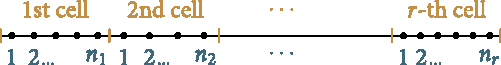
\includegraphics[scale=1.0]{figures/ch_11/fig_11_26.pdf}
		\caption[]{}
		\label{fig:11_26}
	\end{center}
	\vspace{-0.8cm}
\end{figure}

    Các phân tử có thể được phân bố theo các chỗ kí hiệu trên hình \fig{11_26} bằng $N!$ cách ($N!$ là số hoán vị của $N$ phân tử được xếp theo $N$ chỗ). Tuy nhiên, các hoán vị mà nhờ chúng chỉ làm thay đổi thứ tự phân bố các phân tử theo $n_1$ chỗ của ô thứ nhất (số hoán vị này là $n_1!$), hoặc sự phân bố các phân tử theo $n_2$ chỗ của ô thứ hai (số hoán vị này là $n_2!$), vv, không dẫn tới trạng thái vi mô mới. Nhớ rằng các trạng thái vi mô chỉ khác nhau bởi số thứ tự các phân tử rơi vào các ô khác nhau. Cố định số thứ tự của $n_1$ phân tử ở ô thứ nhất. Số hoán vị khác nhau của các phân tử trong ô này tương ứng với mỗi dạng phân bố có thể có của các phân tử còn lại giữa các ô kia là $n_1!$. Do đó, bằng cách chia tổng số hoán vị $N!$ cho $n_1!$, ta loại khỏi việc khảo sát các hoán vị chỉ khác nhau bởi cách phân bố các phân tử trong ô thứ nhất. Sau đó, bằng cách chia $N!/n_1!$ cho $n_2!$, ta loại khỏi việc khảo sát các hoán vị khác nhau bởi cách phân bố các phân tử trong ô thứ hai. Tiếp tục quá trình đó ta đi tới biểu thức
\begin{equation}\label{công thức:11_98}
	\ab{\Omega}{sp} = \frac{N!}{n_1! n_2! \ldots n_r!}
\end{equation}

\noindent
cho ta số phân bố các phân tử theo các ô chỉ khác nhau bởi các số thứ tự khác nhau nằm trong các ô khác nhau [so sánh với \eqn{11_85}]. Số đó là phần "không gian" của trọng số thống kê.

Vì ta đã giả định rằng không có trường ngoại lực, nên ở trạng thái cân bằng, các phân tử được phân bố trên thể tích với mật độ không đổi. Do đó, những con số $n_1, n_2, \ldots, n_r$ về trung bình đều như nhau và bằng $n=N/r$ ($r$ là số ô). Do đó, đối với trạng thái cân bằng, phần "không gian" của trọng số thống kê là
\begin{equation*}
	\ab{\Omega}{sp} = \frac{N!}{(n!)^r}.
\end{equation*}

\noindent
Lấy logarit, ta được
\begin{equation}\label{eq:11_99}
	\ab{\Omega}{sp} = \ln{N!} - r\ln{n!}.
\end{equation}

\noindent
Theo công thức Stirling (see \sect{A_3}), ta được
\begin{equation}\label{eq:11_100}
	\ln{N!} \approx N\ln{N} - N.
\end{equation}

\noindent
Sử dụng công thức \eqn{11_99} ta biến đổi như sau:
\begin{equation*}
	\ln{\ab{\Omega}{sp}} \approx N\ln{N} - N - r(n\ln{n} - N) = N\ln{N} - N\ln{n} = N\ln\parenthesis{\frac{N}{n}}
\end{equation*}

\noindent
(chú ý rằng $rn=N$). The ratio $N/n$ equals $V/\Delta V$. Do đó,
\begin{equation}\label{eq:11_101}
	\ln{\ab{\Omega}{sp}} = N\ln\parenthesis{\frac{V}{\Delta V}} = N\ln{V} - N\ln{\Delta V}.
\end{equation}

Chuyển sang tìn$\ab{\Omega}{v}$. Ta đưa vào không gian các thành phần của vận tốc, các phân tử được đặt theo các trục của không gian đó ($v$-không gian). Ta chia không gian đó thành các ô lập phương như nhau có thể tích $\Delta\Lambda$. Ta sẽ thấy bên dưới rằng giá trị của $\Delta\Lambda$, giống như $\Delta V$ không có ý nghĩa; điều quan trọng là thể tích của $\Delta\Lambda$ đủ lớn sao cho nhiều phân tử "rơi" vào nó.

Ở trạng thái cân bằng, mật độ $\rho$ của các điểm biểu diến vận tốc của các phan tử được xác định bởi hàm phân bố Maxwell [xem công thức \eqref{eq:11_40}, \eqref{eq:11_53}, and~\eqref{eq:11_63}]:
\begin{align*}
	\rho &= N f(v_x, v_y, v_z) = NA^3 \exp\bracket{-\frac{m\parenthesis{v_x^2+v_y^2+v_z^2}}{2kT}}\\
	& = N \parenthesis{\frac{m}{2\pi kT}}^{3/2} \exp\parenthesis{-\frac{mv^2}{2kT}}.
\end{align*}

\noindent
Kí hiệu vận tốc ứng với ô thứ $i$ bằng $\vec{v}_i$ ta thu được giá trị của "mật độ phân tử" trong ô thứ $i$:
\begin{equation*}
	\rho_i = N \parenthesis{\frac{m}{2\pi kT}}^{3/2} \exp\parenthesis{-\frac{mv_i^2}{2kT}}.
\end{equation*}

\noindent
Cuối cùng, nhân mật độ $\rho_i$ với thể tích $\Delta\Lambda$ của ô, ta thu được số phan tử $n_i$ rơi vào ô thứ $i$:
\begin{equation}\label{eq:11_102}
	n_i = N \parenthesis{\frac{m}{2\pi kT}}^{3/2} \exp\parenthesis{-\frac{mv_i^2}{2kT}} \Delta\Lambda.
\end{equation}

\noindent
Tương tự với \eqn{11_98}, ta kết luận rằng số cách mà ta có thể phân phối các phân tử giữa các ô với các giá trị đã cho của các con số là $n_i$ 
\vspace{-12pt} \\
\begin{equation}\label{eq:11_103}
	\ab{\Omega}{v} = \frac{N!}{n_1! n_2! \ldots n_i! \ldots}.
\end{equation}

\noindent
Khác với \eqn{11_98}, số ô bây giờ là vô cùng lớn. Tuy nhiên, đối với các ô đủ cách xa gốc tọa độ, các số $n_i$ thực tế là bằng $0$. Lấy logarit biểu thức \eqn{11_103} ta có
\begin{equation*}
	\ln{\ab{\Omega}{v}} = \ln{N!} - \sum_i \ln{n_i!}.
\end{equation*}

\noindent
Áp dụng công thức\eqref{eq:11_100}, ta được
\begin{equation}\label{eq:11_104}
	\ln{\ab{\Omega}{v}} \approx N\ln{N} - N - \sum_i (n_i \ln{n_i} - n_i) = N\ln{N} - \sum_i n_i\ln{n_i}.
\end{equation}

\noindent
( $\sum_in_i=N$.)

Theo \eqn{11_102}, ta có
\begin{equation*}
	\ln{n_i} = \ln{N} + \ln{\Delta\Lambda} + \frac{3}{2}\ln\parenthesis{\frac{m}{2\pi k}} - \frac{3}{2}\ln{T} - \frac{mv_i^2}{2kT}.
\end{equation*}

\noindent
Đưa phương trình này vào biểu thức \eqref{eq:11_104}, ta được
\begin{multline}
	\ln{\ab{\Omega}{v}} = N\ln{N} - \left(\ln{N} + \ln{\Delta\Lambda} + \frac{3}{2}\ln\parenthesis{\frac{m}{2\pi k}}	\frac{3}{2}\ln{T}\right) \sum_in_i\\
	+ \frac{1}{kT}\sum_i n_i \frac{mv_i^2}{2}.\label{eq:11_105}
\end{multline}

Biểu thức $\sum_in_i\parenthesis{mv_i^2}/2$ tương đương với $N\average{mv^2/2}=3NkT/2$, tổng $\sum_in_i$ bằng $N$. Để ý tới điều đó, ta viết lại \eqn{11_105} như sau:
\begin{align}
	\ln{\ab{\Omega}{v}} &= - N\ln{\Delta\Lambda} - \frac{3}{2} N\ln\parenthesis{\frac{m}{2\pi k}} + \frac{3}{2}N\ln{T} + + \frac{1}{kT}N \frac{3}{2}kT\nonumber\\
	& = \frac{3}{2}N\ln{T} - N\ln{\Delta\Lambda} + \frac{3}{2}N\bracket{1 - \ln\parenthesis{\frac{m}{2\pi k}}}\nonumber\\
	&= \frac{3}{2}N\ln{T} - N\ln{\Delta\Lambda} + \frac{3}{2}N\alpha.\label{eq:11_106}
\end{align}

\noindent
Ở đây $\alpha$ là kí hiệu của biểu thức trong ngoặc không chứa tham số trạng thái của chất khí.

Thế $N$ bằng hằng số Avogadro $\ab{N}{A}$ vào \eqref{eq:11_101} và \eqref{eq:11_106} và sau đó thế các biểu thức đó vào \eqn{11_96}, ta đi đến một công thức cho entropi của một mol khí lý tưởng dạng đơn nguyên tử:
\begin{equation*}
	\ab{S}{m} = k\ab{N}{A}\ln{V} - k\ab{N}{A}\ln{\Delta V} + \frac{3}{2}k\ab{N}{A}\ln{T} - k\ab{N}{A}\ln{\Delta\Lambda} + \frac{3}{2}k\ab{N}{A}\alpha.
\end{equation*}

\noindent
Tích $k\ab{N}{A}$ bằng hằng sô khí $R$. Do đó,
\begin{equation*}
	\ab{S}{m} = R\ln{V} + \frac{3}{2}R\ln{T} - R\ln(\Delta V\Delta\Lambda) + \frac{3}{2}R\alpha.
\end{equation*}

\noindent
Đưa vào kí hiệu
\begin{equation}\label{eq:11_107}
	S_0 = - R\ln(\Delta V\Delta\Lambda) + \frac{3}{2}R\alpha
\end{equation}

\noindent
chú ý rằng $3R/2$ là nhiệt dung phân tử $C_V$ của một khí đơn nguyên tử với thể tích không đổi, ta đi tới công thức cuối cùng
\begin{equation}\label{eq:11_108}
	\ab{S}{m} = R\ln{V} + C_V\ln{T} + S_0.
\end{equation}

\noindent
Công thức này xác định entropy phân tử của chất khí lí tưởng đơn nguyên tử \footnote{$\medskip$Trong~\ref{sec:12_4} sẽ chứng tỏ rằng công thức \eqn{11_108} vẫn đúng cho cả chất khí lí tưởng có các phân tử nhiều nguyên tử.} như hàm của các tham số trạng thái $V$ và $T$. Bằng cách sử dụng một phương trình trạng thái, ta có thể chuyển sang một biểu thức của entropy thông qua các tham số khác, chẳng hạn như $V$ và $p$.

Từ \eqn{11_107} rõ ràng là việc chọn kích thước của các ô $\Delta V$ và $\Delta\Lambda$ chỉ ảnh hưởng tới hằng số cộng tính $S_0$ với độ chính xác mà entropy được xác định bởi công thức \eqn{11_108} đến độ chính xác đó

Khi truyền  cho chất khí một lượng nhiệt $\derivp{Q}$, thì hoặc $T$ thay đổi ($V$ không đổi), hoặc $V$ đổi ($T$ không đổi), hoặc cả $T$ và $V$ đều thay đổi. Một cách tương ứng entropy cũng thay đổi. Để liên hệ sự thay đổi đó với $\derivp{Q}$, ta lấy vi ohana biểu thức \eqn{11_108} và nhân nó với $T$. Kết quả là
\begin{equation*}
	T\,\deriv{\ab{S}{m}} = \frac{RT}{\ab{V}{m}} + C_V\,\deriv{T}
\end{equation*}

\noindent
(để nhấn mạnh rằng ta chú ý đến một mol khí, ta đã đặt cho $V$ chỉ số "M").

Số hạng $C_V\,\deriv{T}$ cho số gia của nội năng chất khí $\deriv{\ab{U}{m}}$. Giả sử quá trình truyền nhiệt $\derivp{Q}$ là quá trình thuận nghịch, có thể biểu diễ số hạng $(RT/\ab{V}{m})\,\deriv{\ab{V}{m}}$ dưới dạng $p\,\deriv{\ab{V}{m}}=\derivp{A}$. Như vậy, ta đi tới hệ thức
\begin{equation*}
	T\,\deriv{\ab{S}{m}} = p\,\deriv{\ab{V}{m}} + \deriv{\ab{U}{m}}.
\end{equation*}

\noindent
Do tính cộng hưởng của $S$, $V$, và $U$, ta có hệ thức tương đối với một lượng khí tùy ý:
\begin{equation*}
	T\,\deriv{S} = p\,\deriv{V} + \deriv{U} = \derivp{A} + \deriv{U}.
\end{equation*}

\noindent
Theo nguyên lí thứ nhất của nhiệt động học, vế phải của đẳng thức này là $\derivp{Q}$. Do đó,
\begin{equation*}
	T\,\deriv{S} = \derivp{Q}.
\end{equation*}

\noindent
Từ đây,
\begin{equation}\label{eq:11_109}
	T\,\deriv{\ab{S}{m. id}} = \frac{\derivp{Q}}{T}\,\,\text{quá trình thuận nghịch}
\end{equation}

\noindent
(Chỉ số "đơn" có nghĩa là chất khí lí tưởng đơn nguyên tử).

Ta đã thu được công thức \eqn{11_109} khi xem xét một khí lý tưởng có dạng cấu tạo. Tuy nhiên, thật đơn giản để mở rộng nó cho bất kỳ hệ thống nhiệt động lực học nào. Giả sử rằng ta có một hệ cô lập ở trạng thái cân bằng mà thành phần của nó, ngoài khí lý tưởng về mặt cấu tạo, bao gồm các thể khác mà sự kết hợp của chúng mà chúng ta gọi là hệ con. Tất cả các bộ phận của hệ thống có cùng nhiệt độ (nếu không trạng thái của hệ thống sẽ không phải là trạng thái cân bằng). Do tính cộng được biểu diễn entropy của hệ $\ab{S}{syst}$ dưới dạng
\begin{equation*}
	\ab{S}{syst} = \ab{S}{sub} + \ab{S}{m. id}
\end{equation*}

\noindent
trong đó $\ab{S}{sub}$ là entropy của hệ con, và $\ab{S}{m. id}$ là entropy của chất khí đơn nguyên tử. Giả sử rằng nhiệt độ của khí có một dao động vô cùng nhỏ $\deriv{T}$. Do đó, chất khí nhận từ hệ con nhiệt lượng $\derivp{\ab{Q}{m. id}}$. Đồng thời hệ con nhận nhiệt lượng $\derivp{\ab{Q}{sub}}=-\derivp{\ab{Q}{m. id}}$. Vì $\deriv{T}$ bé có thể xem quá trình đó là thuận nghich. Do đó entropy của chất khí nhân số gia $\deriv{\ab{S}{m. id}}=\derivp{\ab{Q}{m. id}}/T$.

Khi một quá trình thuận nghịch xảy ra trong một hệ cô lập, entropi của hệ không đổi. Do đó, nó theo sau 
\begin{equation*}
	\deriv{\ab{S}{syst}} = \deriv{\ab{S}{sub}} + \deriv{\ab{S}{m. id}} = 0.
\end{equation*}

\noindent
Tính đến giá trị của $\deriv{\ab{S}{m. id}}$, đối với số gia entropy của hệ con ta thu được biểu thức:
\begin{equation*}
	\deriv{\ab{S}{sub}} = -\deriv{\ab{S}{m. id}} = -\frac{\derivp{\ab{Q}{m. id}}}{T} = \frac{\derivp{\ab{Q}{sub}}}{T}.
\end{equation*}

\noindent
Do đó, đối với các vật tập hợp tùy ý, ta có công thức
\begin{equation}\label{eq:11_110}
	\deriv{S} = \frac{\derivp{Q}}{T}
\end{equation}

\noindent
Ở đây $\derivp{Q}$ là lượng nhiệt mà hệ thu được trong quá trình thuận nghịch, và $T$ là nhiệt độ của hệ.

Lưu ý rằng trong khi $\derivp{Q}$không phải là một vi phân toàn phần thì biểu thức \eqn{11_110} là một vi phân toàn phần (entropy là hàm trạng thái).

Bây giờ có thể giải thích tại sao trong công thức \eqn{11_93}, hằng số Boltzmann $k$ được lấy làm hệ số tỉ lệ. Do đó, người ta đã thu được hệ số tỉ lệ giữa $\deriv{S}$ và $\derivp{Q}/T$ là bằng đươn vị [xem \eqn{11_110}].

Trạng thái được thực hiện bởi một số cách tương đối nhỏ được gọi là \textbf{trạng thái trật tự} hoặc \textbf{trạng thái không ngẫu nhiên}. Trạng thái được thực hiện theo nhiều cách khác nhau được gọi là \textbf{trạng thái hỗn loạn} hoặc \textbf {trạng thái ngẫu nhiên}. Do đó, entropy là một thước đo định lượng về mức độ rối loạn phân tử trong một hệ. Trường hợp này giúp bạn có thể hiểu được ý nghĩa của \eqn{11_110}. Việc cung cấp nhiệt cho một hệ thống dẫn đến chuyển động nhiệt lớn hơn của các phân tử và do đó, làm tăng mức độ rối loạn trong hệ. Nhiệt độ càng cao, tức là nội năng của hệ càng lớn, thì phần rối loạn tương đối nhỏ hơn do cung cấp nhiệt lượng đã cho $\derivp{Q}$.

Tính đúng đắn của quá trình trong đó nhiệt lượng $\derivp{Q}$ được cung cấp cho hệ là điều kiện quan trọng để \eqn{11_110} duy trì. Nếu lượng nhiệt $\derivp{Q}$ được truyền cho hệ trong quá trình không thuận nghịch, thì entropy phát triển do cung cấp nhiệt và do quá trình không thuận nghịch. Do đó, ta có bất đẳng thức.
\begin{equation}\label{eq:11_111}
	\deriv{S} > \frac{\derivp{Q}}{T}.\,\, \text{quá trình không thuận nghịch}
\end{equation}

\noindent
Khi $\derivp{Q}$ biến mất, bất đẳng thức này chuyển thành biểu thức \eqref{eq: 11_94}. Theo công thức $T$ trong công thức \eqref{eq: 11_111}, được hiểu ngầm là nhiệt độ của bể chứa mà từ đó hệ đã cho thu được nhiệt lượng $\derivp{Q}$. Nhiệt độ của hệ trong một quá trình không thuận nghịch có thể không có giá trị xác định vì trạng thái của hệ không phải là trạng thái cân bằng.

Ta có thể gộp các công thức \eqn{11_110} và \eqn{11_111} lại với nhau bằng cách viết:
\begin{equation}\label{eq:11_112}
	\deriv{S} \geqslant \frac{\derivp{Q}}{T}.
\end{equation}

\noindent
Dấu đẳng thức liên quan đến các quá trình thuận nghịch và dấu bất đẳng liên quan đến các quá trình không thuận nghịch.

Hệ thức \eqref{eq:11_112} là nền tảng cho các ứng dụng nhiệt động lực học của khái niệm entropy. Những ứng dụng này sẽ được giải quyết trong chương sau.

Ở độ không tuyệt đối, như thường lệ, như một quy tắc \footnote{$\medskip$Các ngoại lệ mà ta sẽ không đề cập đến thường xảy ra ngoài quy tắc đó.}, Ở trạng thái cơ bản của nó có trọng số thống kê bằng thống nhất ($\Omega=1$). Phương trình  \eqref{eq:11_93} cho giá trị bằng 0 đối với entropy trong trường hợp này. Do đó, nó dẫn đến việc \textbf{khi nhiệt độ của một vật có xu hướng bằng không tuyệt đối, entropy của nó có xu hướng bằng không}:
\begin{equation}\label{eq:11_113}
	\lim_{T\to 0} S = 0.
\end{equation}

\noindent
Khẳng định này là nội dung của định lí \textbf{Nernst}. Đôi khi khẳng định trên được gọi là \textbf{nguyên lí thứ ba của nhiệt động học}.
